\documentclass[conference]{IEEEtran}
\IEEEoverridecommandlockouts
% The preceding line is only needed to identify funding in the first footnote. If that is unneeded, please comment it out.
\usepackage{cite}
\usepackage{amsmath,amssymb,amsfonts}
\usepackage{algorithmic}
\usepackage{graphicx}
\usepackage{textcomp}
\usepackage{xcolor}
\usepackage{booktabs}
\usepackage{multirow}
\usepackage{url}
\usepackage{hyperref}

\def\BibTeX{{\rm B\kern-.05em{\sc i\kern-.025em b}\kern-.08em
    T\kern-.1667em\lower.7ex\hbox{E}\kern-.125emX}}

\begin{document}

\title{CarbonAI: An Explainable Extreme Gradient Boosting and Tool-Augmented Conversational Framework for Real-Time Industrial Carbon Intelligence}

\author{
\IEEEauthorblockN{SHINAGAM RANJITH KUMAR}
\IEEEauthorblockA{\textit{Computer Science and Engineering} \\
\textit{VIT-AP University}\\
Amaravathi, India}
\and
\IEEEauthorblockN{THAMMINANA VIPUL}
\IEEEauthorblockA{\textit{Computer Science and Engineering} \\
\textit{VIT-AP University}\\
Amaravathi, India}
\and
\IEEEauthorblockN{PRANAY KUMAR}
\IEEEauthorblockA{\textit{Computer Science and Engineering} \\
\textit{VIT-AP University}\\
Amaravathi, India}
}

\maketitle

\begin{center}
\small
\textbf{Guide: Dr. Afzal Hussain Shahid}\\
Assistant Professor Senior Grade 2\\
School of Computer Science and Engineering (SCOPE)\\
VIT-AP University, Amaravathi, India
\end{center}

\vspace{0.8em}

\begin{abstract}
Industrial decarbonization requires granular, real-time quantification of greenhouse gas emissions coupled with actionable mitigation intelligence. Most conventional carbon accounting methodologies rely on retrospective annual self-reporting and static emissions factors, while existing predictive machine learning models function as isolated black-box estimators that output scalar values without domain context or operational remediation guidance. To overcome these limitations, this paper introduces \textbf{CarbonAI}, an end-to-end cyber-physical intelligence framework that unifies an Extreme Gradient Boosting (XGBoost) regressor with Tree SHAP explainability and a Retrieval-Augmented Generation (RAG) conversational advisor. Trained on an expansive multi-sector dataset of 18,250 industrial facilities spanning manufacturing, agriculture, energy, transport, and information technology, the model incorporates seven domain-engineered physical operational ratios designed to eliminate data leakage. Empirical evaluation on an untouched holdout test partition ($n = 2,738$) demonstrates a coefficient of determination ($R^2$) of 0.8682, a Mean Absolute Error (MAE) of 4.1586 $\text{tCO}_2\text{e}$, a Root Mean Squared Error (RMSE) of 5.2504 $\text{tCO}_2\text{e}$, and an unbiased mean residual of -0.0689 $\text{tCO}_2\text{e}$. Global SHAP attribution confirms non-renewable energy consumption ($\text{mean } |\text{SHAP}| = 9.4825$) and renewable energy share as the primary determinants of carbon variance. Rather than presenting isolated numbers, CarbonAI routes predictions into a FAISS vector store coupled with a Gemini Large Language Model via bidirectional tool execution, enabling real-time counterfactual ``what-if'' simulations and regulatory compliance grounding. Deployed via a scalable FastAPI microservice and ReactJS interface, the platform provides a complete decision-support ecosystem for industrial sustainability engineering.
\end{abstract}

\begin{IEEEkeywords}
Industrial Carbon Intelligence, XGBoost Regressor, Explainable AI (XAI), Tree SHAP, Retrieval-Augmented Generation (RAG), Scope 1--3 Emissions, Decarbonization Decision Support.
\end{IEEEkeywords}

\section{Introduction and Key Contributions}

\subsection{Background}
Anthropogenic greenhouse gas (GHG) emissions originating from industrial manufacturing, thermal power generation, global logistics, and resource extraction remain the dominant catalysts of contemporary climate instability \cite{ghgprotocol2004}, \cite{ritchie2020co2}. Under established frameworks such as the Greenhouse Gas Protocol, industrial enterprises are required to quantify and report their carbon footprint across Scope 1 (direct operational combustion), Scope 2 (indirect emissions from purchased electricity and steam), and Scope 3 (upstream and downstream supply chain logistics) \cite{ghgprotocol2004}. Historically, organizational carbon accounting has operated as an annualized, retrospective auditing exercise. Facility managers aggregate utility billing records and fuel consumption logs, subsequently multiplying these totals by standardized, region-averaged emissions factors \cite{liu2022survey}.

However, conventional accounting regimes suffer from catastrophic latency: emission totals are finalized months after the physical operations have ceased, entirely precluding proactive intervention or dynamic load-shifting. In response, modern data science and industrial Internet of Things (IIoT) telemetry have enabled automated, machine learning-driven emissions estimation \cite{tiwari2023cyber}. By mapping high-frequency operational signals---such as electricity consumption, fossil fuel throughput, raw material feed rates, transport distances, and workforce scale---supervised learning algorithms can approximate carbon intensity in near real time \cite{aras2022interpretable}, \cite{chen2022lca}.

Within predictive analytics, gradient-boosted decision tree ensembles, specifically Extreme Gradient Boosting (XGBoost), have emerged as the premier paradigm for tabular telemetry data \cite{chen2016xgboost}. By sequentially constructing shallow decision trees that minimize regularized objective functions, gradient boosting models effectively navigate complex non-linear interactions, heteroscedastic noise, and multicollinearity without requiring prohibitive computational infrastructure \cite{friedman2001greedy}.

\subsection{Problem Definition}
Despite significant advances in predictive accuracy, existing computational carbon estimation frameworks suffer from two fundamental systemic vulnerabilities:

\textit{1) The Opaque Black-Box Silo}: High-dimensional machine learning regressors output solitary scalar predictions (e.g., ``42.8 $\text{tCO}_2\text{e}$''). They fail to articulate \textit{why} a given facility generated that footprint, what operational bottlenecks contributed to the observed variance, or how local variables interacted \cite{ribeiro2016lime}, \cite{molnar2022interpretable}. Without rigorous, mathematically grounded explainability, industrial engineers and compliance auditors cannot safely trust or act upon model predictions \cite{osei2023trust}.

\textit{2) The Disconnect Between Diagnosis and Decarbonization Guidance}: Estimating emissions is merely the first operational requirement; the paramount agronomic or engineering utility lies in identifying viable remediation pathways \cite{savary2022digital}. Off-the-shelf generative Large Language Models (LLMs) possess vast domain knowledge but suffer from severe hallucinations when asked to calculate emissions or evaluate specialized facility trade-offs \cite{lewis2020rag}, \cite{gao2023ragreview}. Conversely, static rule-based engines lack conversational adaptability.

To bridge this structural gap, this research introduces \textbf{CarbonAI}, an integrated cyber-physical intelligence platform that explicitly couples an explainable XGBoost regressor with a tool-augmented Retrieval-Augmented Generation (RAG) conversational pipeline. By tethering generative language reasoning to verified vector embeddings of corporate sustainability directives and equipping the LLM with direct function-calling execution of the underlying machine learning model, CarbonAI converts static predictions into dynamic, verified decarbonization roadmaps.

\subsection{Key Contributions}
The primary contributions of this paper are summarized as follows:
\begin{enumerate}
    \item \textbf{High-Fidelity Tabular Carbon Regressor}: We engineer and train an optimized XGBoost model on 18,250 multi-sector industrial facility records across five major economic sectors (Manufacturing, Agriculture, Energy, Transport, IT) and four critical industrial sub-sectors (Steel, Cement, Automotive, Logistics). The model achieves an $R^2$ of 0.8682, an MAE of 4.1586 $\text{tCO}_2\text{e}$, and an RMSE of 5.2504 $\text{tCO}_2\text{e}$ on unseen test data.
    \item \textbf{Leakage-Free Physical Feature Engineering}: We formulate seven non-leaking operational intensity metrics (e.g., Non-Renewable Energy per Unit Production, Renewable Energy Share, Transport Intensity, and Energy per Employee) while systematically eliminating 11 confounding and post-prediction leakage variables (such as target-derived carbon taxes).
    \item \textbf{Auditable Feature Explainability via Exact Tree SHAP}: We implement exact Tree SHAP (SHapley Additive exPlanations) attribution to mathematically decompose global feature importance and provide facility-level marginal directional impact breakdowns for every inference.
    \item \textbf{Tool-Augmented Conversational RAG Architecture}: We construct a dual-layer conversational advisor integrating FAISS dense vector retrieval (`all-MiniLM-L6-v2`) with a Gemini LLM equipped with four callable Python tools. This enables the chatbot to run real-time ``what-if'' simulations directly on the XGBoost inference graph rather than hallucinating outputs.
    \item \textbf{Production-Grade Full-Stack SaaS Deployment}: We package the entire pipeline into a scalable FastAPI REST microservice with SQLite persistence, JWT authentication, automated CSV schema adaptation, and an interactive ReactJS frontend.
\end{enumerate}

\begin{figure}[htbp]
\centering
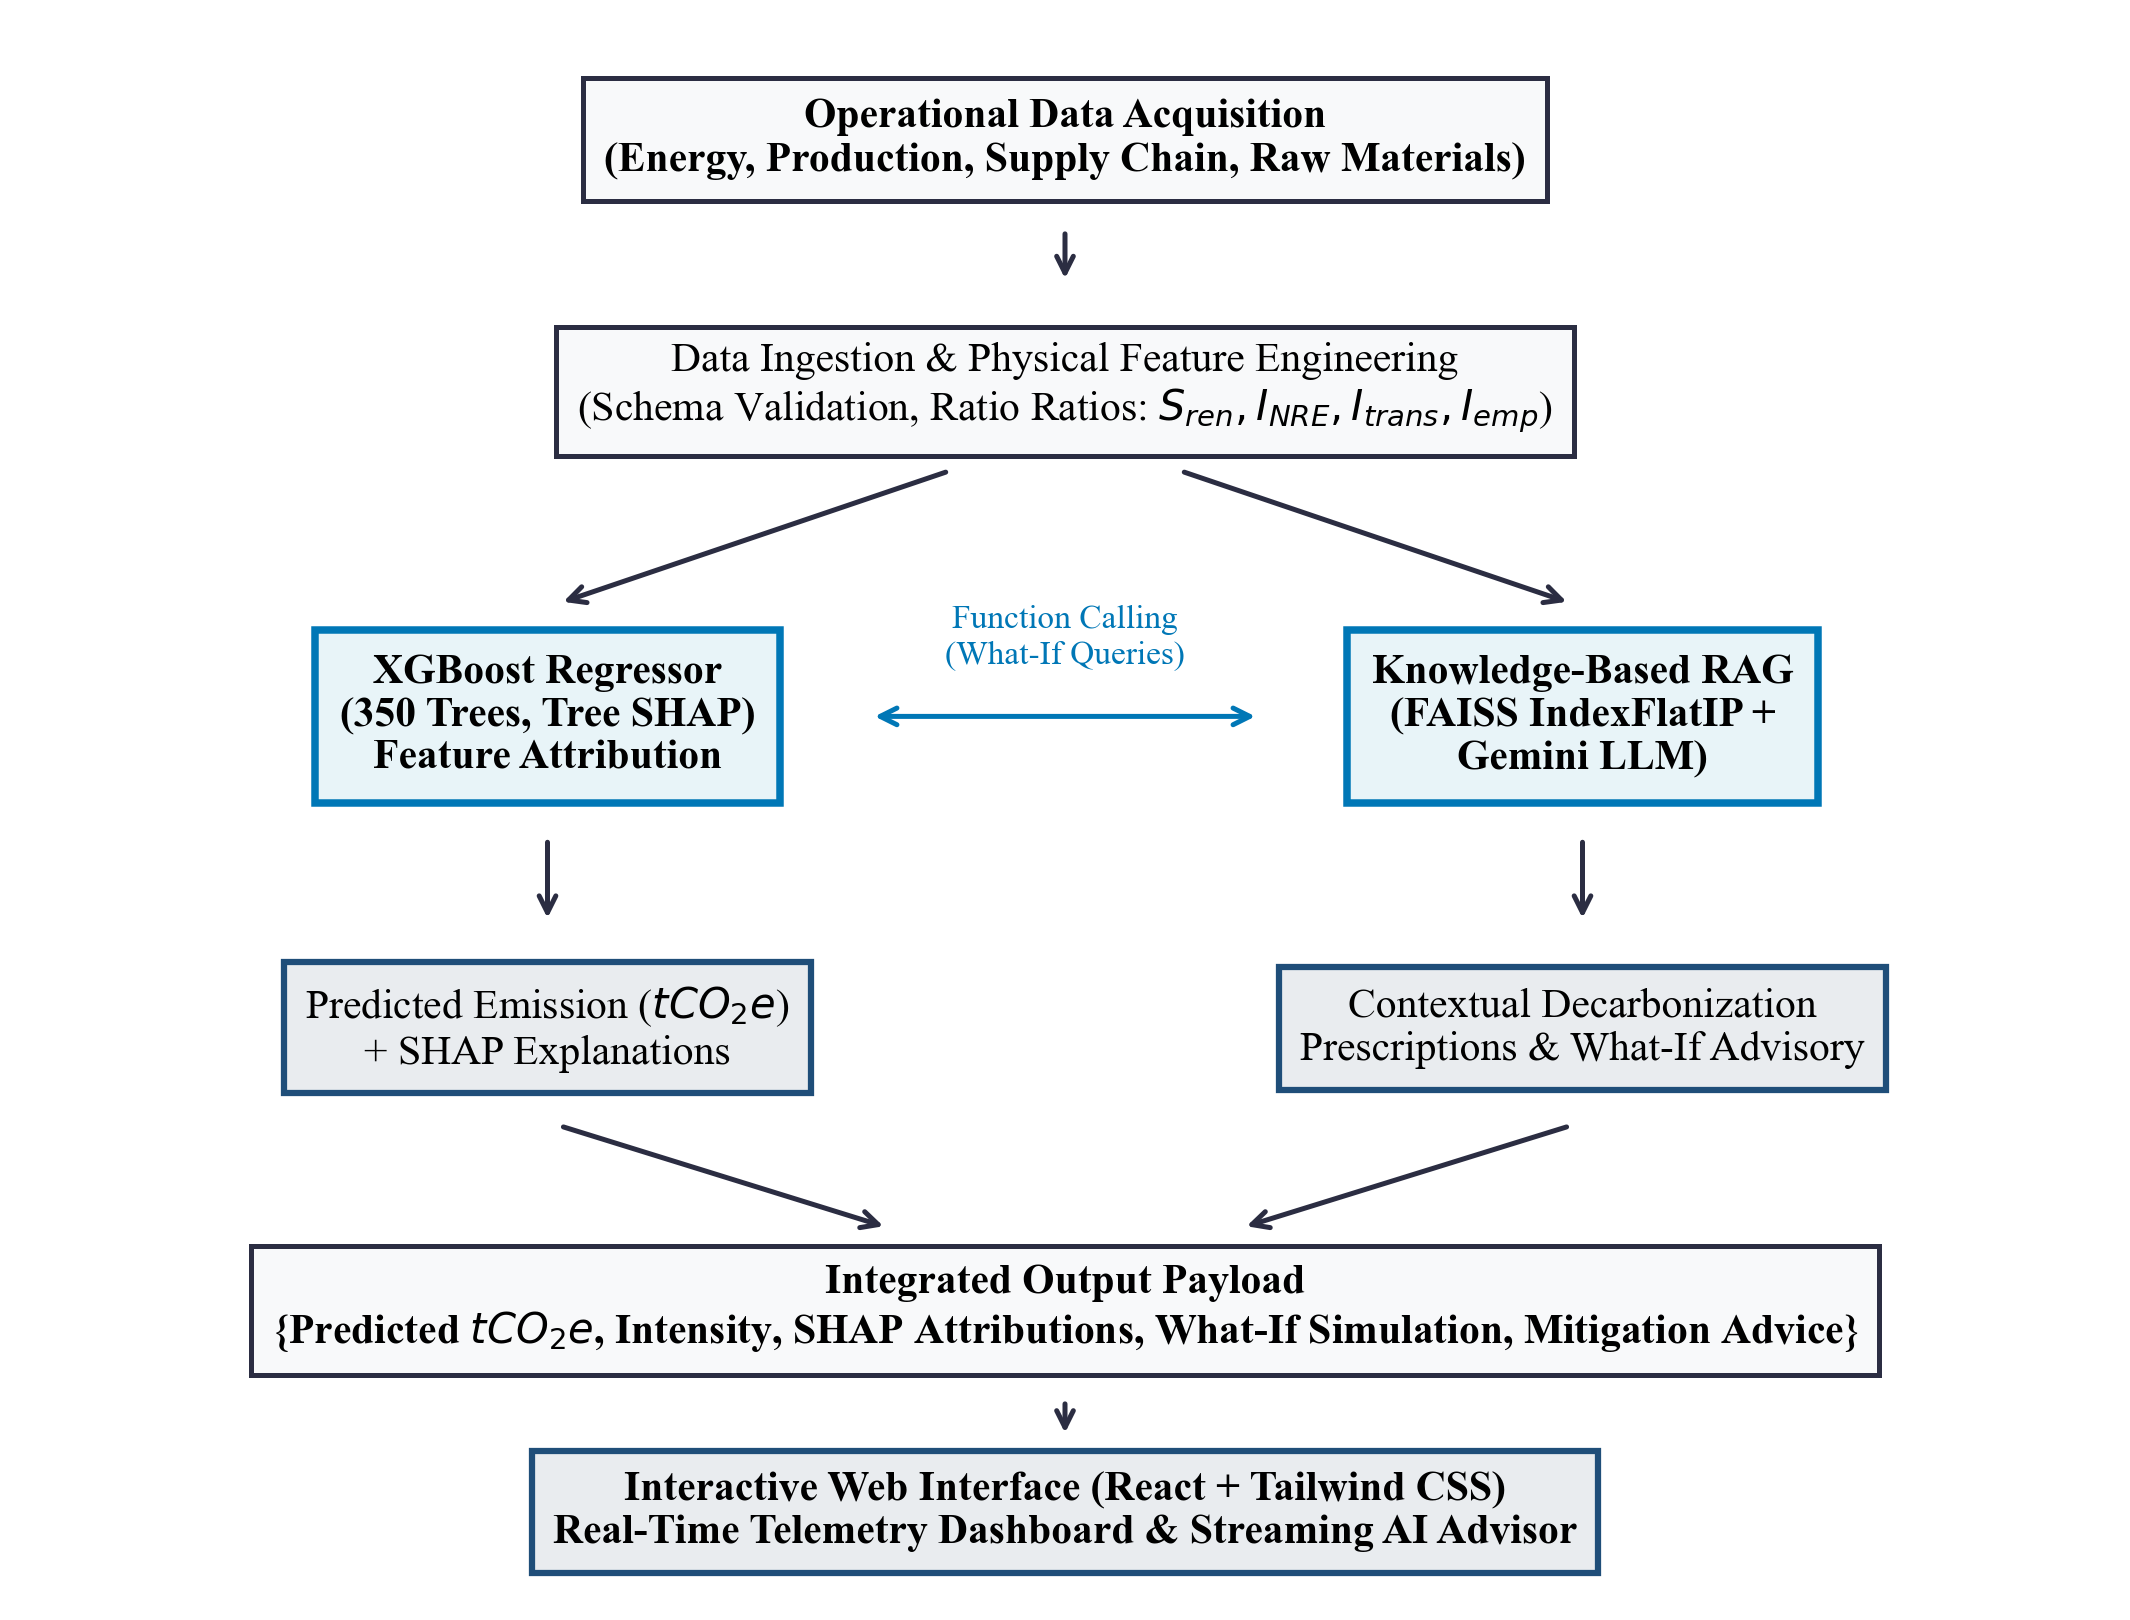
\includegraphics[width=\columnwidth]{Figures/fig1_workflow.png}
\caption{Workflow of the proposed hybrid CarbonAI architecture.}
\label{fig:workflow}
\end{figure}

\section{Literature Review}

The trajectory of automated industrial emissions modeling has evolved through multiple distinct methodological phases, progressing from basic statistical inventories to complex deep neural networks and multimodal reasoning agents.

\subsection{Statistical Inventories and Machine Learning Baselines}
Early emissions quantification depended primarily on empirical linear regression models and IPCC Tier 1/2 emission factors \cite{ghgprotocol2004}. While computationally trivial, these approaches assumed constant linear scalability between production volume and carbon output, disregarding vital operational variables such as fuel switching, partial capacity operations, and seasonal grid emission factor fluctuations \cite{liu2022survey}.

With the proliferation of factory automation, researchers applied classical machine learning algorithms, including Support Vector Regression (SVR) \cite{drucker1996svr} and Random Forests (RF) \cite{breiman2001random}, to capture non-linearities in industrial energy consumption \cite{aras2022interpretable}. For instance, Chen et al. demonstrated that ensemble tree models outperformed linear benchmarks by over 24\% in predicting manufacturing product life cycle emissions \cite{chen2022lca}. However, standard random forests often struggle with high-dimensional sparse categorical feature spaces and lack native regularization mechanisms against noisy industrial telemetry.

\subsection{Gradient Boosting and Deep Learning in Carbon Modeling}
The introduction of Extreme Gradient Boosting (XGBoost) marked a notable milestone in tabular data modeling \cite{chen2016xgboost}. By utilizing exact second-order Taylor expansions of the loss function, depth-wise tree pruning, and integrated $L_1$ and $L_2$ leaf weight regularization, XGBoost routinely eclipses deep artificial neural networks (ANNs) on structured industrial tabular datasets \cite{aras2022interpretable}, \cite{fang2023energy}. Recent investigations by Zhao et al. \cite{zhao2024carbon} and Zhao and Wang \cite{zhao2025forecasting} confirmed that gradient-boosted topologies achieve superior generalization in carbon time-series forecasting while avoiding the severe overfitting and immense hyperparameter sensitivity typical of recurrent neural networks.

\subsection{Explainable Artificial Intelligence (XAI) in Energy Systems}
As machine learning models are increasingly integrated into regulatory reporting and carbon tax compliance frameworks, model opacity has emerged as a significant technical and legal liability \cite{wu2025carbonquant}. Traditional feature importance metrics (e.g., Gini impurity decrease or split frequency) suffer from severe bias toward continuous variables with high cardinality \cite{molnar2022interpretable}.

To establish mathematical rigor, cooperative game theory was introduced via Shapley Additive exPlanations (SHAP) \cite{lundberg2017unified}. Lundberg et al. formulated Tree SHAP, an algorithm that evaluates exact conditional expectation Shapley values in low-order polynomial time $\mathcal{O}(TLD^2)$ rather than exponential time \cite{lundberg2020nature}. In industrial decarbonization studies, Fang et al. demonstrated that SHAP values allow plant managers to isolate the exact marginal impact of specific fuel-switching initiatives \cite{fang2023energy}.

\subsection{Retrieval-Augmented Generation (RAG) and Agentic LLMs}
Despite their predictive capabilities, supervised regression models remain isolated diagnostic calculators: they cannot interpret corporate decarbonization mandates, compare results against municipal regulations, or converse with facility operators \cite{gao2023ragreview}. Conversely, general-purpose Large Language Models (LLMs) \cite{vaswani2017attention} possess broad semantic comprehension but cannot perform dependable quantitative arithmetic or access private enterprise documentation \cite{lewis2020rag}.

The Retrieval-Augmented Generation (RAG) paradigm resolves this dichotomy by anchoring LLMs to vetted external knowledge repositories \cite{lewis2020rag}. Utilizing dense vector embeddings (e.g., Sentence-BERT \cite{reimers2019sentence}) indexed via high-performance similarity search algorithms like Facebook AI Similarity Search (FAISS) \cite{johnson2021faiss}, RAG pipelines dynamically extract relevant policy chunks to ground language generation. CarbonAI extends this paradigm by introducing bidirectional tool calling: the conversational agent not only retrieves static policy excerpts but directly triggers the compiled XGBoost inference graph to evaluate live ``what-if'' engineering scenarios.

\begin{figure*}[htbp]
\centering
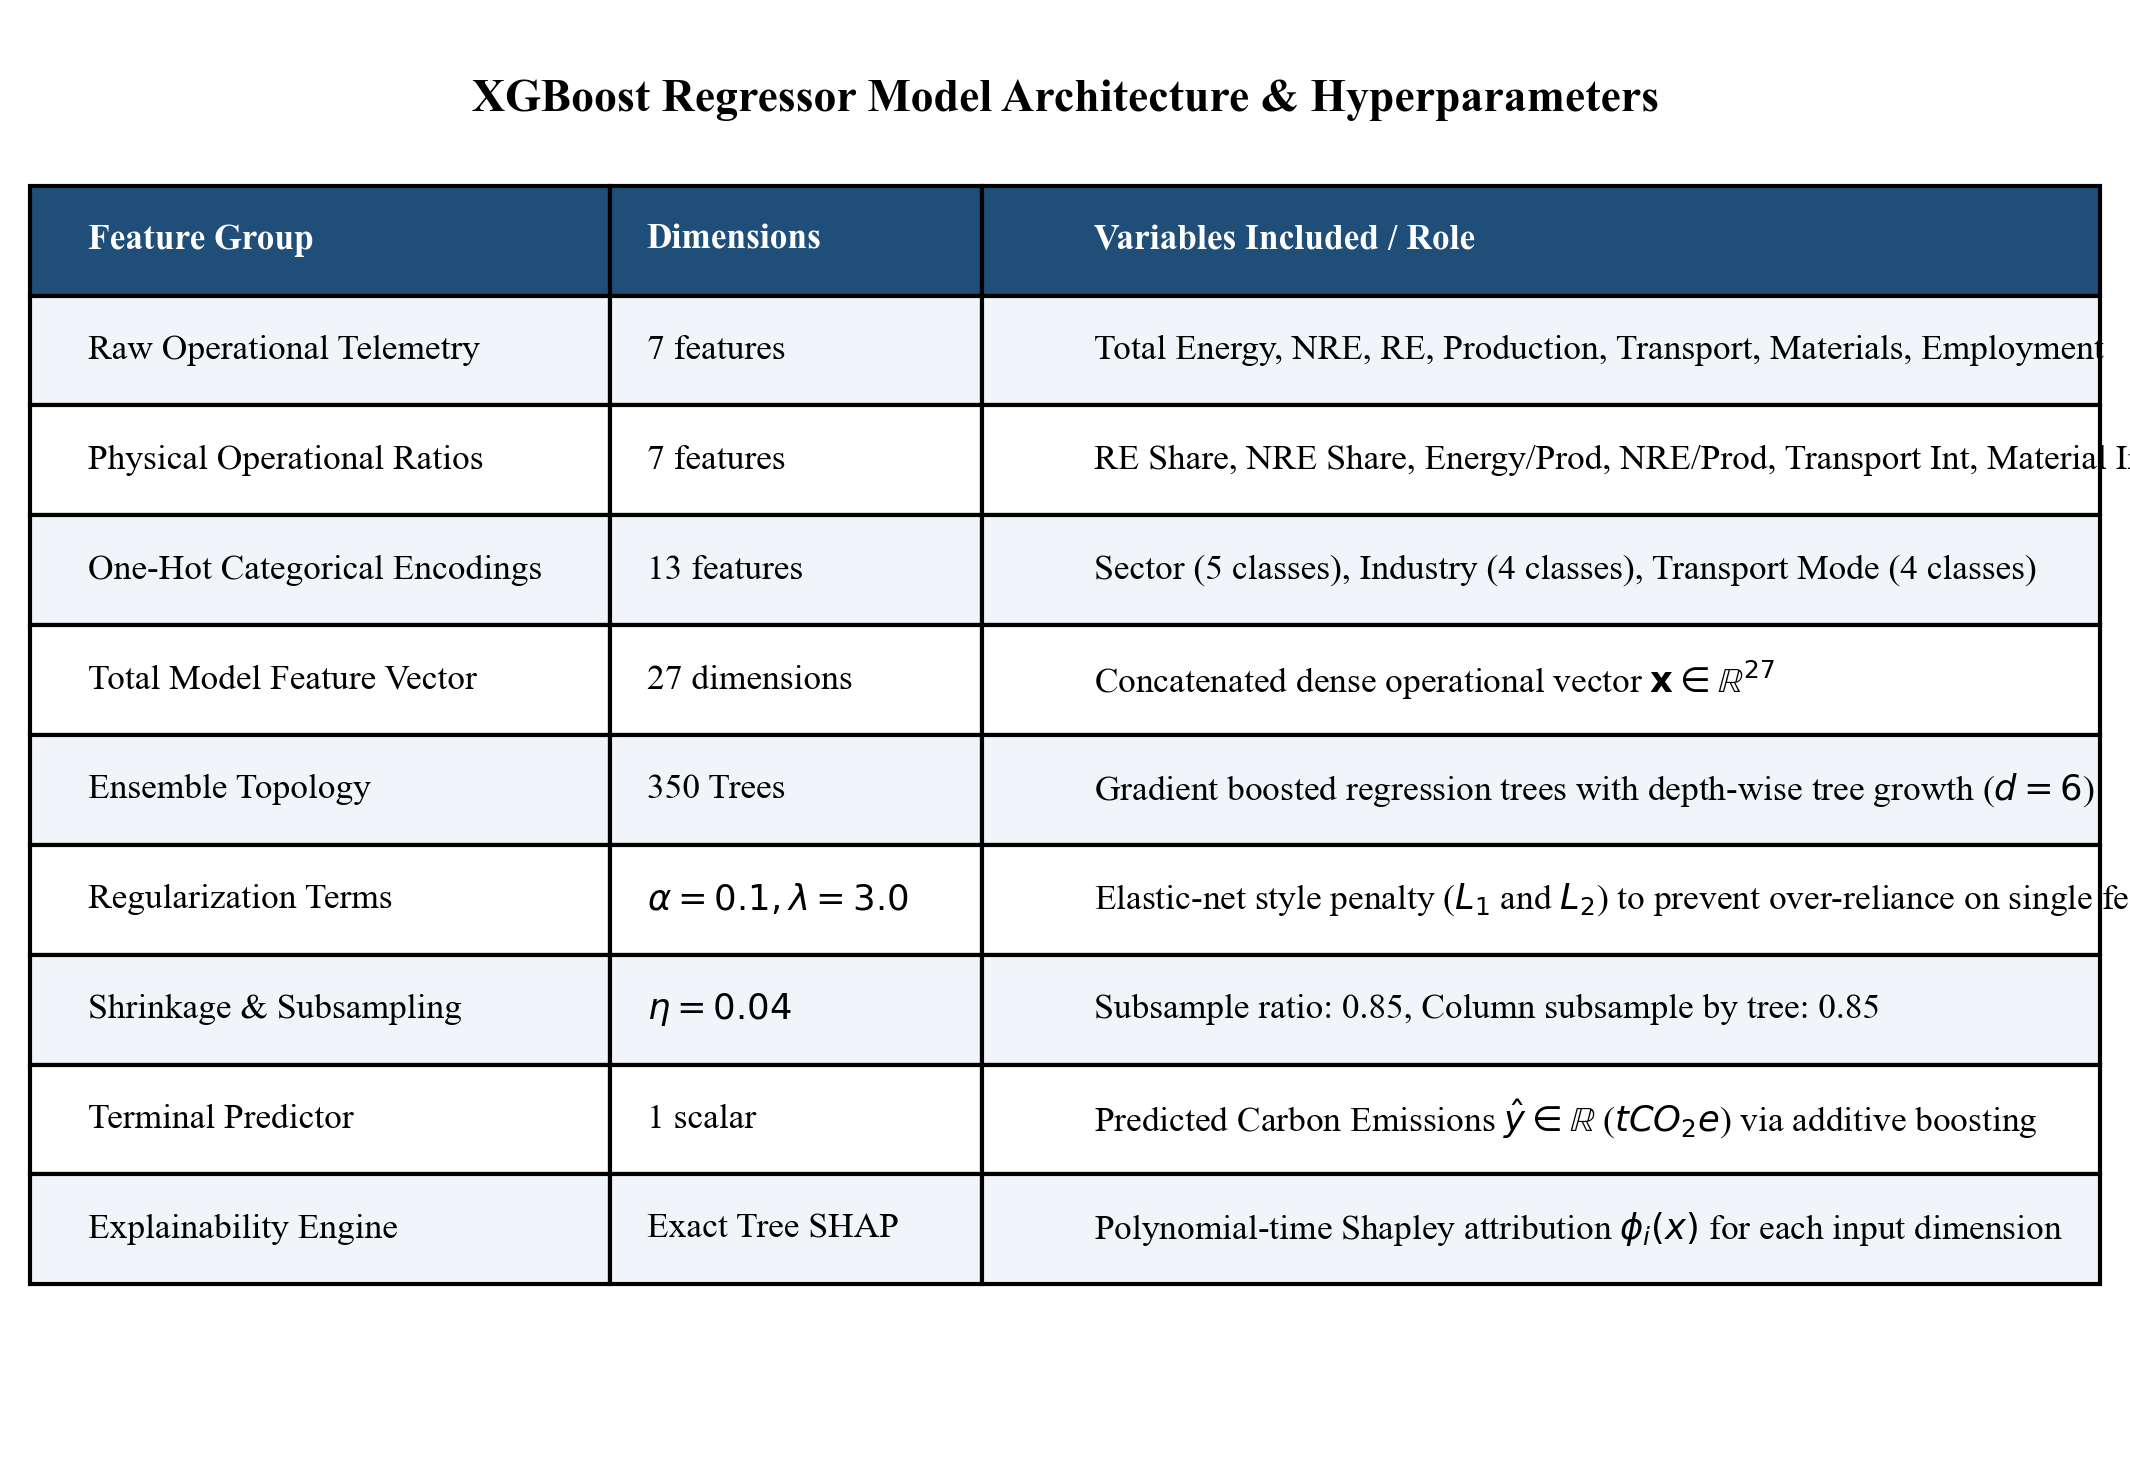
\includegraphics[width=0.92\textwidth]{Figures/fig2_model_architecture.png}
\caption{XGBoost Regressor model architecture, feature space composition, and hyperparameter configuration.}
\label{fig:model_arch}
\end{figure*}

\section{Proposed Methodology}

\subsection{Overall Architecture}
The proposed CarbonAI platform is organized into three interconnected operational subsystems:
\begin{enumerate}
    \item \textbf{The Data Processing and Feature Engineering Module}: Ingests raw facility metrics, validates schemas, enforces data leakage boundaries, and derives non-linear physical intensity indicators.
    \item \textbf{The Predictive and Explainability Core}: Executes gradient boosted regression via an optimized XGBoost engine, followed by local and global feature attribution via exact Tree SHAP.
    \item \textbf{The Tool-Augmented Conversational RAG Advisor}: Indexes unstructured sustainability documentation within FAISS and leverages Gemini LLM function-calling capabilities to provide grounded decarbonization recommendations.
\end{enumerate}

The complete system workflow is illustrated in Fig.~\ref{fig:workflow}, demonstrating the end-to-end data pipeline from user input to unified JSON output.

\subsection{Mathematical Foundation of the XGBoost Regressor}
Let the training dataset be denoted as $\mathcal{D} = \{(\mathbf{x}_i, y_i)\}_{i=1}^N$, where $\mathbf{x}_i \in \mathbb{R}^M$ represents the $M$-dimensional feature vector for facility $i$, and $y_i \in \mathbb{R}^+$ denotes the ground-truth carbon emissions measured in metric tonnes of $\text{CO}_2$ equivalent ($\text{tCO}_2\text{e}$).

The ensemble model generates the predicted emission $\hat{y}_i$ via an additive combination of $K$ regression trees:
\begin{equation}
\hat{y}_i = \phi(\mathbf{x}_i) = \sum_{k=1}^K f_k(\mathbf{x}_i), \quad f_k \in \mathcal{F}
\label{eq:additive}
\end{equation}
where $\mathcal{F} = \{f(\mathbf{x}) = w_{q(\mathbf{x})}\} \; (q: \mathbb{R}^M \to T, \; \mathbf{w} \in \mathbb{R}^T)$ denotes the space of Classification and Regression Trees (CART). Here, $q$ defines the tree's decision structure mapping a sample to its corresponding leaf index, $T$ is the total leaf count, and $\mathbf{w}$ represents the vector of continuous leaf weights.

To prevent overfitting while minimizing empirical error, the regularized objective function $\mathcal{L}$ is formulated as:
\begin{equation}
\mathcal{L}(\phi) = \sum_{i=1}^N l(y_i, \hat{y}_i) + \sum_{k=1}^K \Omega(f_k)
\label{eq:objective}
\end{equation}
where $l$ is the differentiable squared error loss function $l(y_i, \hat{y}_i) = \frac{1}{2}(y_i - \hat{y}_i)^2$, and $\Omega(f_k)$ penalizes model complexity via:
\begin{equation}
\Omega(f_k) = \gamma T + \alpha \sum_{j=1}^T |w_j| + \frac{1}{2}\lambda \sum_{j=1}^T w_j^2
\label{eq:regularization}
\end{equation}
Here, $\gamma$ represents the complexity penalty for adding an extra leaf, while $\alpha$ and $\lambda$ denote the $L_1$ (Lasso) and $L_2$ (Ridge) regularization parameters on leaf weights, respectively.

At step $t$, the objective function is iteratively approximated using a second-order Taylor expansion around the prediction at step $t-1$:
\begin{equation}
\mathcal{L}^{(t)} \approx \sum_{i=1}^N \left[ l(y_i, \hat{y}_i^{(t-1)}) + g_i f_t(\mathbf{x}_i) + \frac{1}{2} h_i f_t^2(\mathbf{x}_i) \right] + \Omega(f_t)
\label{eq:taylor}
\end{equation}
where the first-order gradient $g_i$ and second-order Hessian $h_i$ are defined as:
\begin{equation}
g_i = \partial_{\hat{y}^{(t-1)}} l(y_i, \hat{y}^{(t-1)}) = (\hat{y}_i^{(t-1)} - y_i)
\end{equation}
\begin{equation}
h_i = \partial_{\hat{y}^{(t-1)}}^2 l(y_i, \hat{y}^{(t-1)}) = 1
\end{equation}

For a given leaf $j$, let $I_j = \{i \mid q(\mathbf{x}_i) = j\}$ denote the instance set mapped to that leaf. By setting the partial derivative $\frac{\partial \mathcal{L}^{(t)}}{\partial w_j} = 0$, the optimal leaf weight $w_j^*$ is derived analytically:
\begin{equation}
w_j^* = -\frac{\sum_{i \in I_j} g_i}{\sum_{i \in I_j} h_i + \lambda}
\label{eq:optimal_weight}
\end{equation}

Substituting $w_j^*$ back into the objective yields the minimal loss score for evaluating tree structure quality:
\begin{equation}
\tilde{\mathcal{L}}^{(t)}(q) = -\frac{1}{2} \sum_{j=1}^T \frac{\left(\sum_{i \in I_j} g_i\right)^2}{\sum_{i \in I_j} h_i + \lambda} + \gamma T
\end{equation}

During node splitting, the score gain obtained by partitioning a parent node instance set $I = I_L \cup I_R$ into left ($I_L$) and right ($I_R$) child nodes is computed as:
\begin{equation}
\mathcal{L}_{\text{split}} = \frac{1}{2}\left[ \frac{\left(\sum_{i \in I_L} g_i\right)^2}{\sum_{i \in I_L} h_i + \lambda} + \frac{\left(\sum_{i \in I_R} g_i\right)^2}{\sum_{i \in I_R} h_i + \lambda} - \frac{\left(\sum_{i \in I} g_i\right)^2}{\sum_{i \in I} h_i + \lambda} \right] - \gamma
\label{eq:gain}
\end{equation}

\subsection{Physical Operational Feature Engineering}
To capture realistic physical intensity dynamics, the seven raw numeric metrics ($E_{\text{total}}$, $E_{\text{ren}}$, $E_{\text{nonren}}$, $P$, $D_{\text{trans}}$, $M_{\text{raw}}$, $L$) are transformed into seven operational ratios, incorporating clipping boundaries to guarantee numerical stability:
\begin{equation}
S_{\text{ren}} = \min\left(1.0, \max\left(0.0, \frac{E_{\text{ren}}}{\max(E_{\text{total}}, 1.0)}\right)\right)
\end{equation}
\begin{equation}
S_{\text{nonren}} = \min\left(1.0, \max\left(0.0, \frac{E_{\text{nonren}}}{\max(E_{\text{total}}, 1.0)}\right)\right)
\end{equation}
\begin{equation}
I_E = \frac{E_{\text{total}}}{\max(P, 1.0)}, \quad I_{\text{NRE}} = \frac{E_{\text{nonren}}}{\max(P, 1.0)}
\end{equation}
\begin{equation}
I_{\text{trans}} = \frac{D_{\text{trans}}}{\max(P, 1.0)}, \quad I_{\text{mat}} = \frac{M_{\text{raw}}}{\max(P, 1.0)}
\end{equation}
\begin{equation}
I_{\text{emp}} = \frac{E_{\text{total}}}{\max(L, 1.0)}
\end{equation}
Together with 13 one-hot encoded categorical indicators representing economic Sector, Industry Sector, and Transport Mode, the final feature space comprises $M = 27$ dimensions (detailed in Fig.~\ref{fig:model_arch}).

\subsection{Tree SHAP Explainability Formulation}
To guarantee local accuracy, missingness, and consistency, model predictions are interpreted via Shapley values grounded in cooperative game theory \cite{lundberg2017unified}. The prediction for sample $\mathbf{x}$ is decomposed as an additive attribution sum:
\begin{equation}
\hat{y}(\mathbf{x}) = \phi_0 + \sum_{m=1}^M \phi_m(\mathbf{x})
\label{eq:shap_additive}
\end{equation}
where $\phi_0 = \mathbb{E}[\hat{y}(\mathbf{x})]$ is the expected base value across the background training population, and $\phi_m(\mathbf{x})$ is the marginal contribution of feature $m$, calculated via:
\begin{equation}
\phi_m(\mathbf{x}) = \sum_{S \subseteq \mathcal{M} \setminus \{m\}} \frac{|S|!(M - |S| - 1)!}{M!} \left[ f_x(S \cup \{m\}) - f_x(S) \right]
\end{equation}
Global feature importance is evaluated by computing the mean absolute Shapley attribution across the evaluation cohort:
\begin{equation}
I_m = \frac{1}{N} \sum_{i=1}^N |\phi_m(\mathbf{x}_i)|
\end{equation}

\begin{figure}[htbp]
\centering
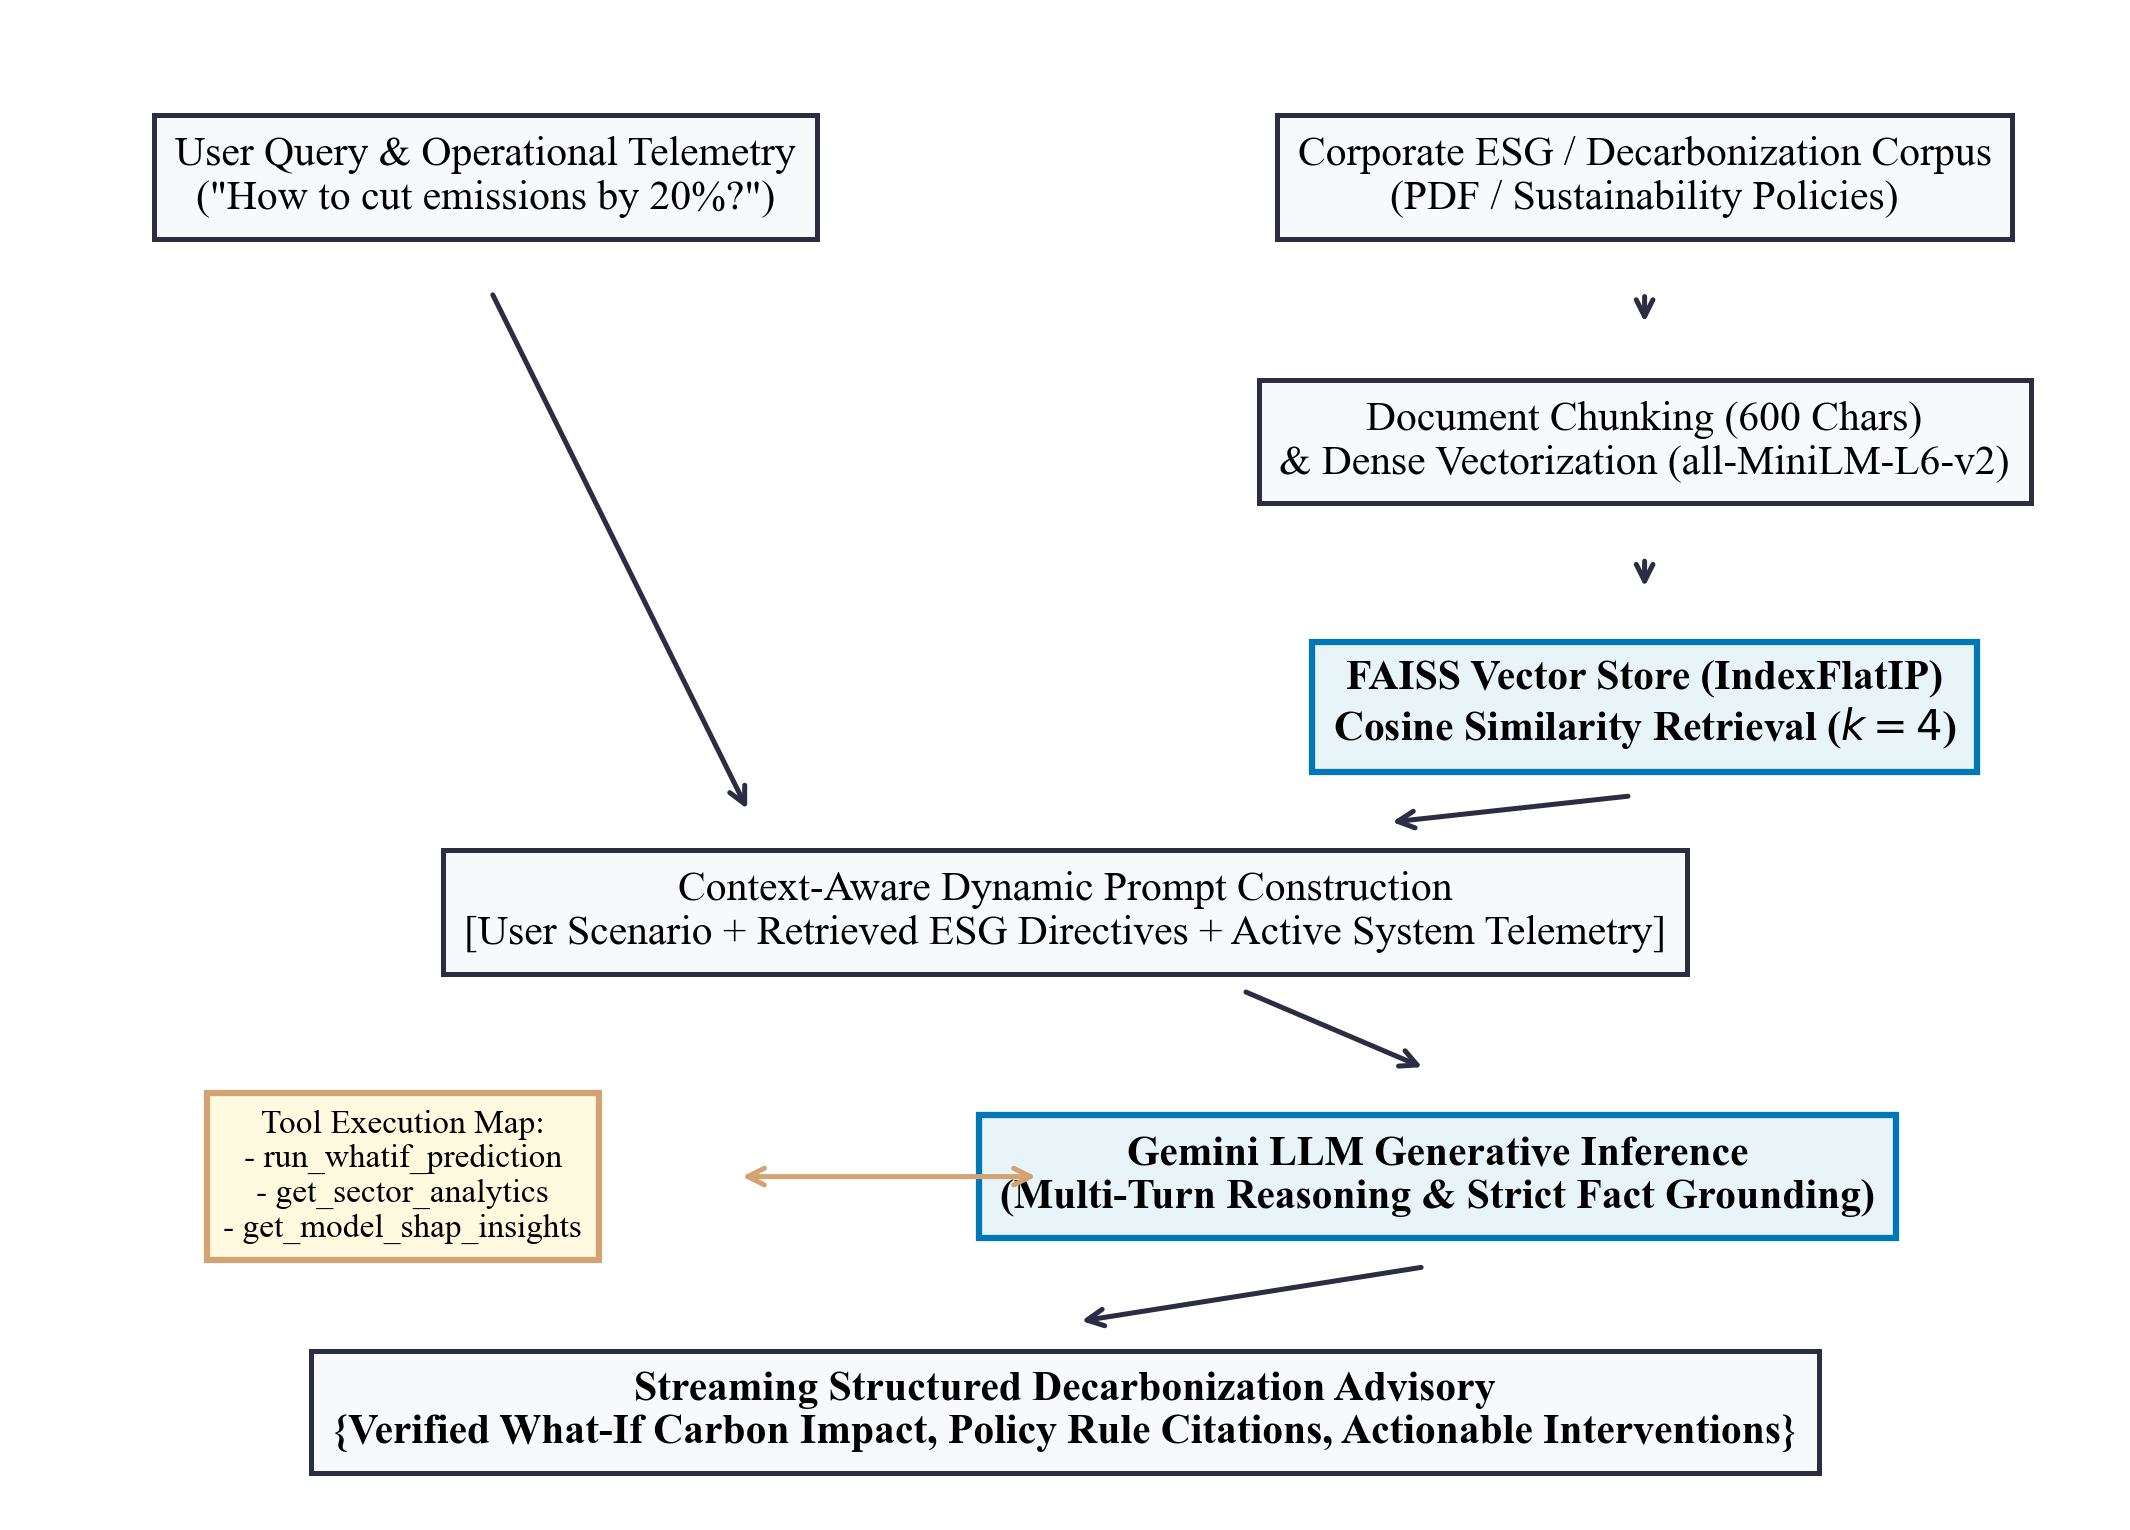
\includegraphics[width=\columnwidth]{Figures/fig3_rag_pipeline.png}
\caption{Architecture of the RAG-driven conversational advisory pipeline.}
\label{fig:rag_pipeline}
\end{figure}

\subsection{Knowledge-Based Conversational RAG Pipeline}
The conversational subsystem contextualizes the numerical outputs of the XGBoost regressor against unstructured corporate policies and environmental guidelines (e.g., ISO 14064, corporate internal carbon prices, and Scope 3 reduction goals). As depicted in Fig.~\ref{fig:rag_pipeline}, the pipeline operates as follows:

\textit{1) Document Ingestion and Vectorization}: Corporate sustainability PDFs or text documents are parsed into overlapping chunks $d_i$ of length 600 characters with a 100-character stride. Each chunk is mapped into a continuous 384-dimensional dense semantic vector space using the Sentence-BERT model `all-MiniLM-L6-v2`:
\begin{equation}
\mathbf{v}_i = \mathcal{E}(d_i) \in \mathbb{R}^{384}, \quad \|\mathbf{v}_i\|_2 = 1
\end{equation}

\textit{2) FAISS Dense Vector Indexing}: Vectors are indexed in a Facebook AI Similarity Search (FAISS) `IndexFlatIP` structure. Upon receiving a natural language query $q$, the query vector $\mathbf{v}_q = \mathcal{E}(q)$ is evaluated against all indexed vectors via inner product cosine similarity:
\begin{equation}
\text{sim}(\mathbf{v}_q, \mathbf{v}_i) = \mathbf{v}_q \cdot \mathbf{v}_i = \cos(\theta)
\end{equation}
The top-$k$ most semantically relevant policy chunks ($k=4$) are extracted to construct the context prompt $\mathcal{C} = \{d_{(1)}, \dots, d_{(k)}\}$.

\textit{3) Tool-Augmented Generative Inference}: Rather than permitting the Large Language Model (Gemini 3.6/3.5 Flash) to generate speculative carbon figures, the agent is bounded by four registered Python execution tools:
\begin{itemize}
    \item `run_whatif_prediction`: Dispatches counterfactual operational scenarios directly to the XGBoost inference graph.
    \item `get_sector_and_dataset_analytics`: Retrieves cross-sector benchmark statistics and average emission baselines.
    \item `get_model_and_shap_insights`: Returns verified model test metrics ($R^2$, MAE, RMSE) and top SHAP drivers.
    \item `get_my_recent_predictions`: Queries historical facility simulation logs from the persistent SQLite database.
\end{itemize}

\begin{figure}[htbp]
\centering
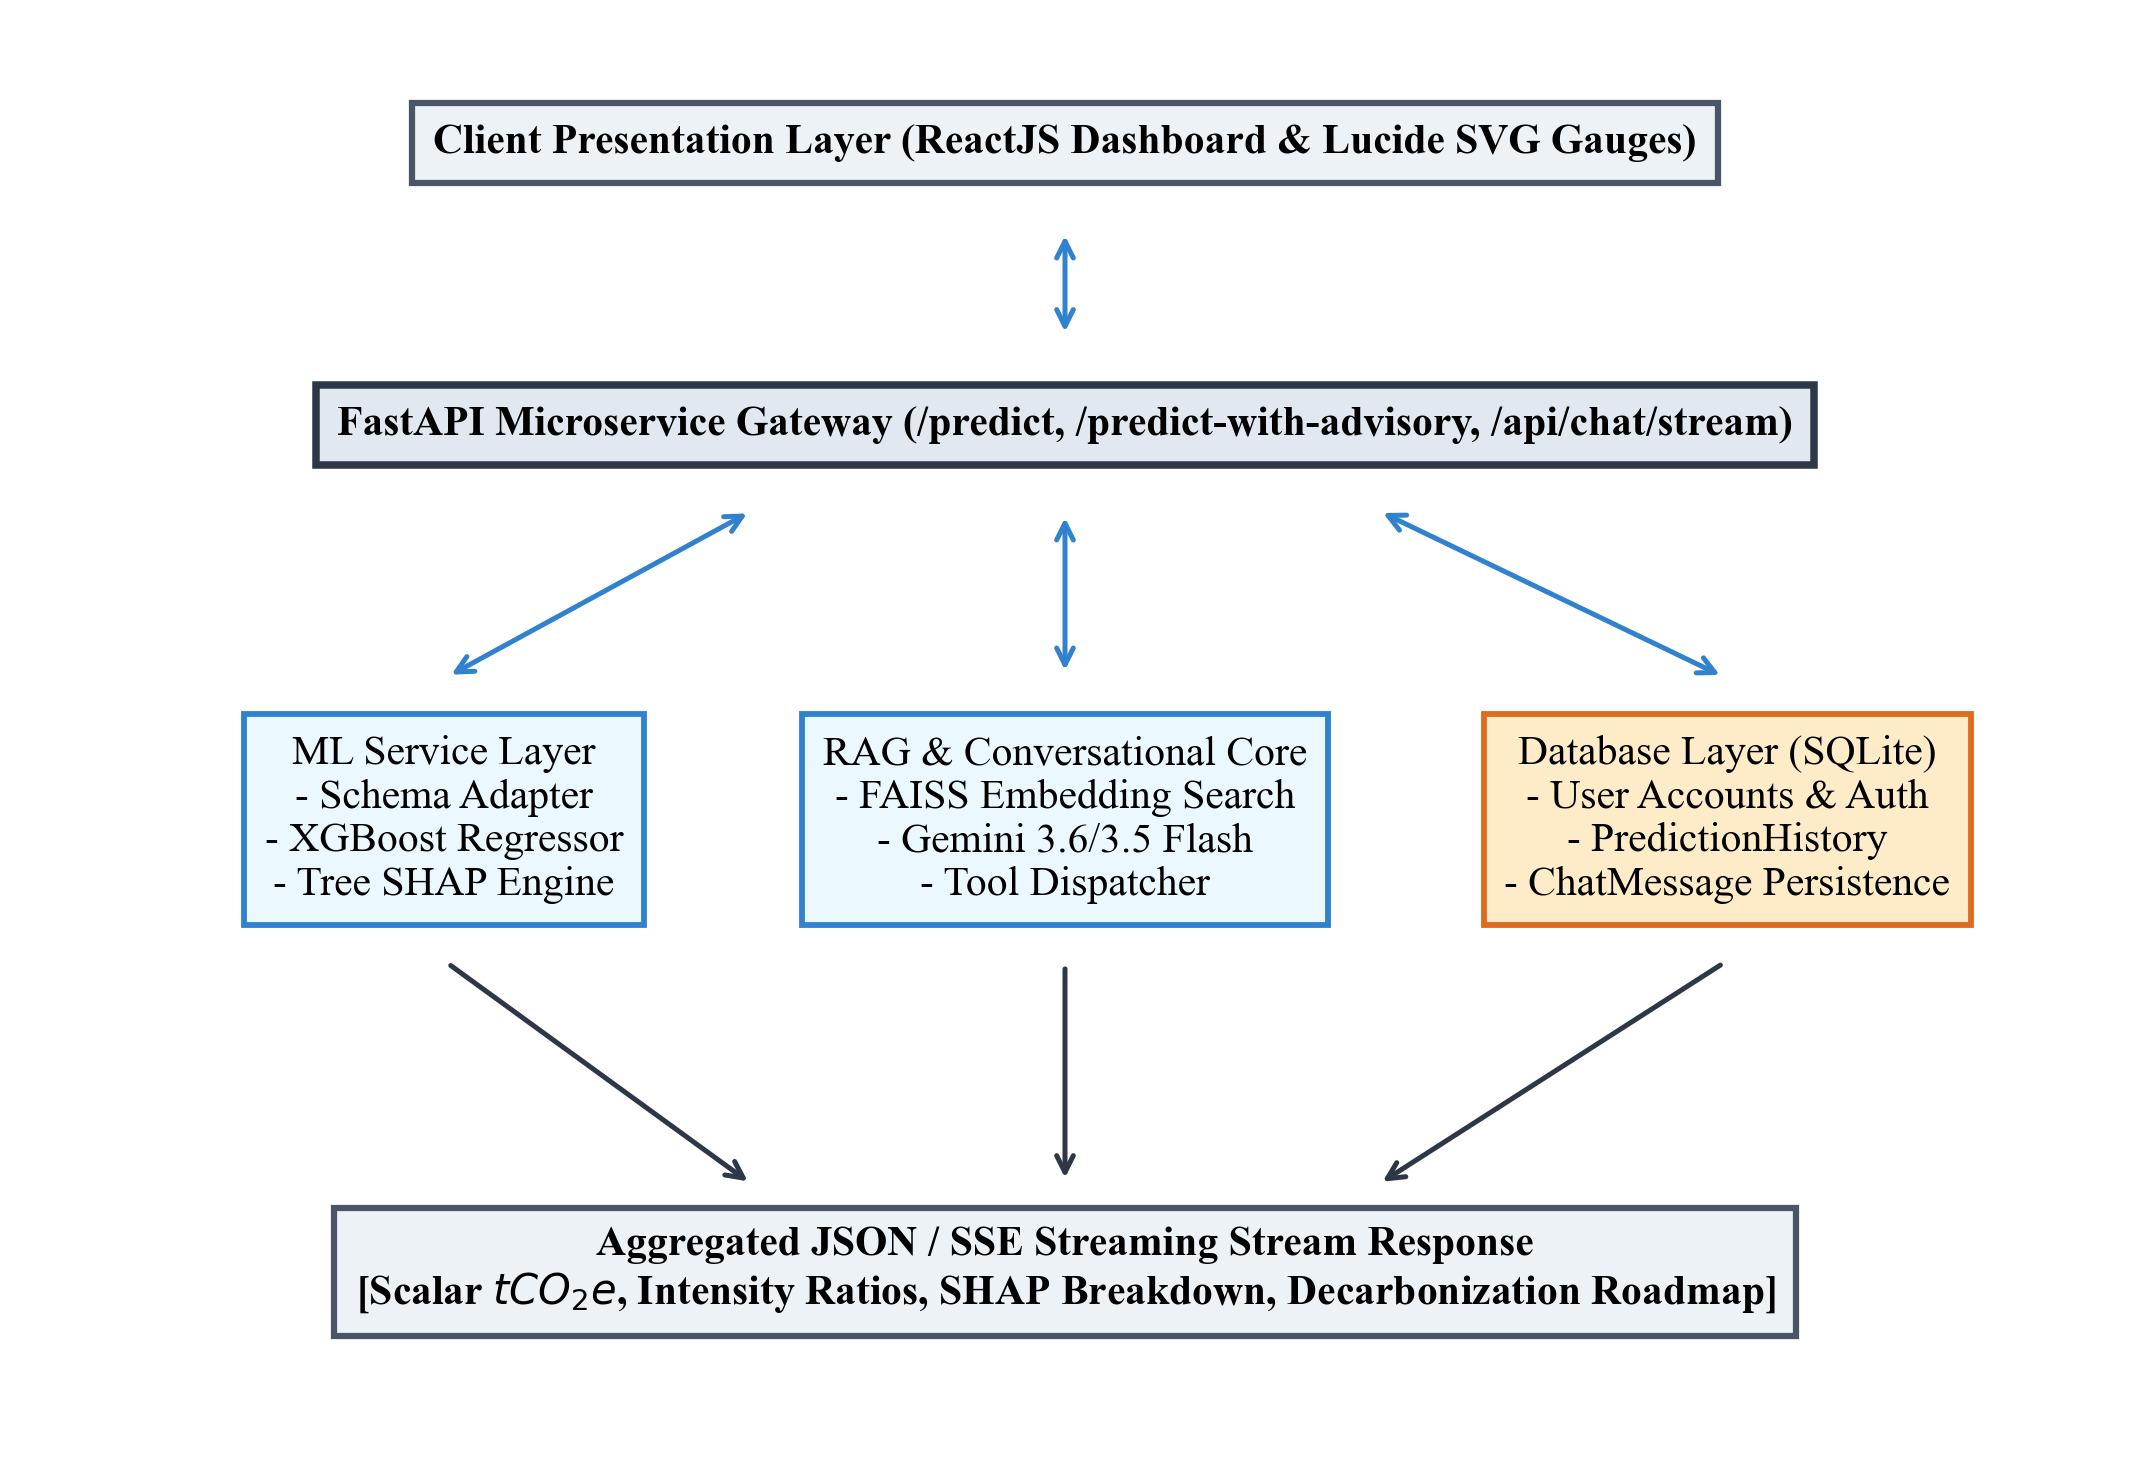
\includegraphics[width=\columnwidth]{Figures/fig4_data_flow.png}
\caption{End-to-end data flow within the hybrid FastAPI deployment.}
\label{fig:data_flow}
\end{figure}

\subsection{Integration and Data Flow}
Fig.~\ref{fig:data_flow} outlines the end-to-end software integration. The presentation layer, built with ReactJS, provides interactive operational sliders, dynamic SVG gauges, and a streaming chat drawer. Telemetry payloads are transmitted over HTTP to a FastAPI gateway. The gateway invokes the model service, records simulation records in SQLite via SQLAlchemy ORM, and triggers Server-Sent Events (SSE) streaming for multi-turn conversational responses.

\begin{table}[htbp]
\caption{Dataset Partitioning and Distribution}
\begin{center}
\begin{tabular}{lcc}
\toprule
\textbf{Split Partition} & \textbf{Number of Facilities} & \textbf{Percentage} \\
\midrule
Training Set             & 12,775                         & 70.0\% \\
Validation Set           & 2,737                          & 15.0\% \\
Holdout Test Set         & 2,738                          & 15.0\% \\
\midrule
\textbf{Total Dataset}   & \textbf{18,250}                & \textbf{100.0\%} \\
\bottomrule
\end{tabular}
\label{tab:splits}
\end{center}
\end{table}

\begin{figure}[htbp]
\centering
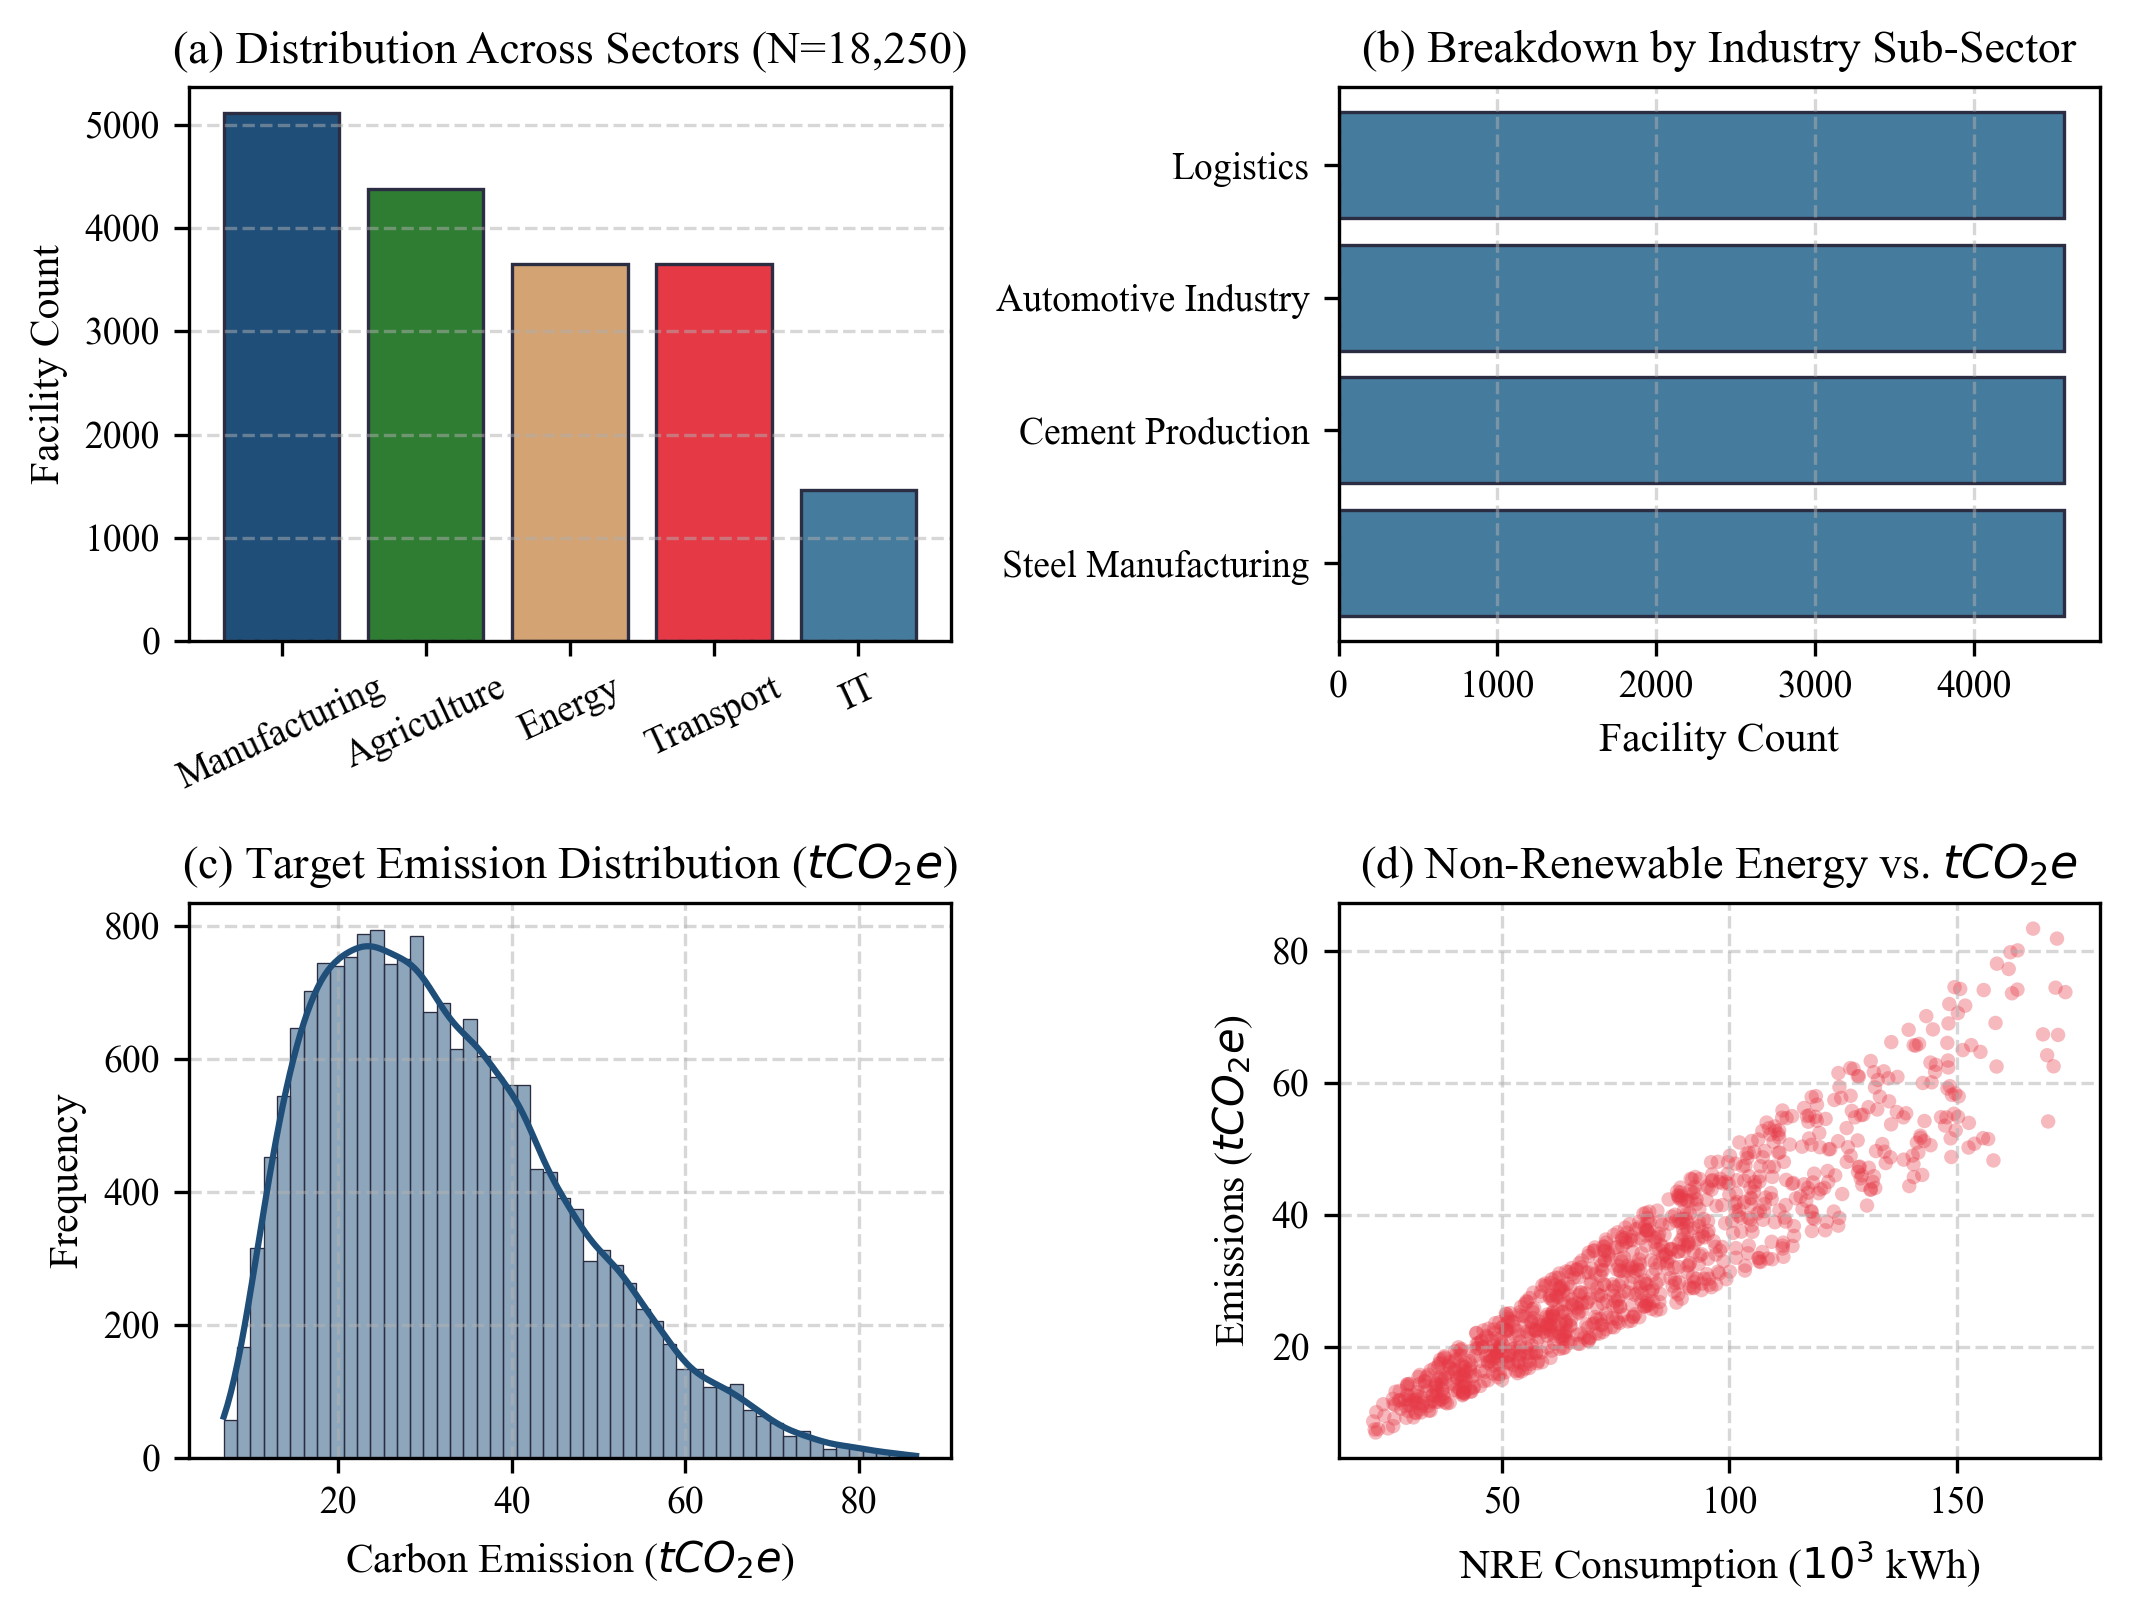
\includegraphics[width=\columnwidth]{Figures/fig5_dataset_distributions.png}
\caption{Dataset distributions across industrial sectors and operational features.}
\label{fig:dataset_dist}
\end{figure}

\section{Experimental Results and Discussions}

\subsection{Dataset Description and Preprocessing}
The experimental validation of CarbonAI was performed on a dataset comprising 18,250 unique industrial facility operational records. The corpus encompasses five economic sectors: Manufacturing ($n=5,110$, 28.0\%), Agriculture ($n=4,380$, 24.0\%), Energy ($n=3,650$, 20.0\%), Transport ($n=3,650$, 20.0\%), and Information Technology ($n=1,460$, 8.0\%). Within heavy industry, four specialized sub-sectors are represented in balanced proportions: Steel Manufacturing (4,563 facilities), Cement Production (4,563 facilities), Automotive Industry (4,562 facilities), and Logistics (4,562 facilities). Furthermore, four supply chain transport modes are captured: Ship (4,581), Air (4,567), Truck (4,559), and Rail (4,543).

As presented in Table~\ref{tab:splits}, the dataset was partitioned using a strict, reproducible random split into 70\% training ($n=12,775$), 15\% validation ($n=2,737$), and 15\% untouched holdout testing ($n=2,738$). Fig.~\ref{fig:dataset_dist} illustrates the multi-panel distributions of sectors, sub-sectors, target carbon emissions ($t\text{CO}_2\text{e}$), and non-renewable energy consumption. The continuous target variable spans from $0.00$ to $86.57\text{ tCO}_2\text{e}$, exhibiting a unimodal distribution with a mean of $31.84\text{ tCO}_2\text{e}$ and standard deviation of $14.47\text{ tCO}_2\text{e}$.

\begin{figure}[htbp]
\centering
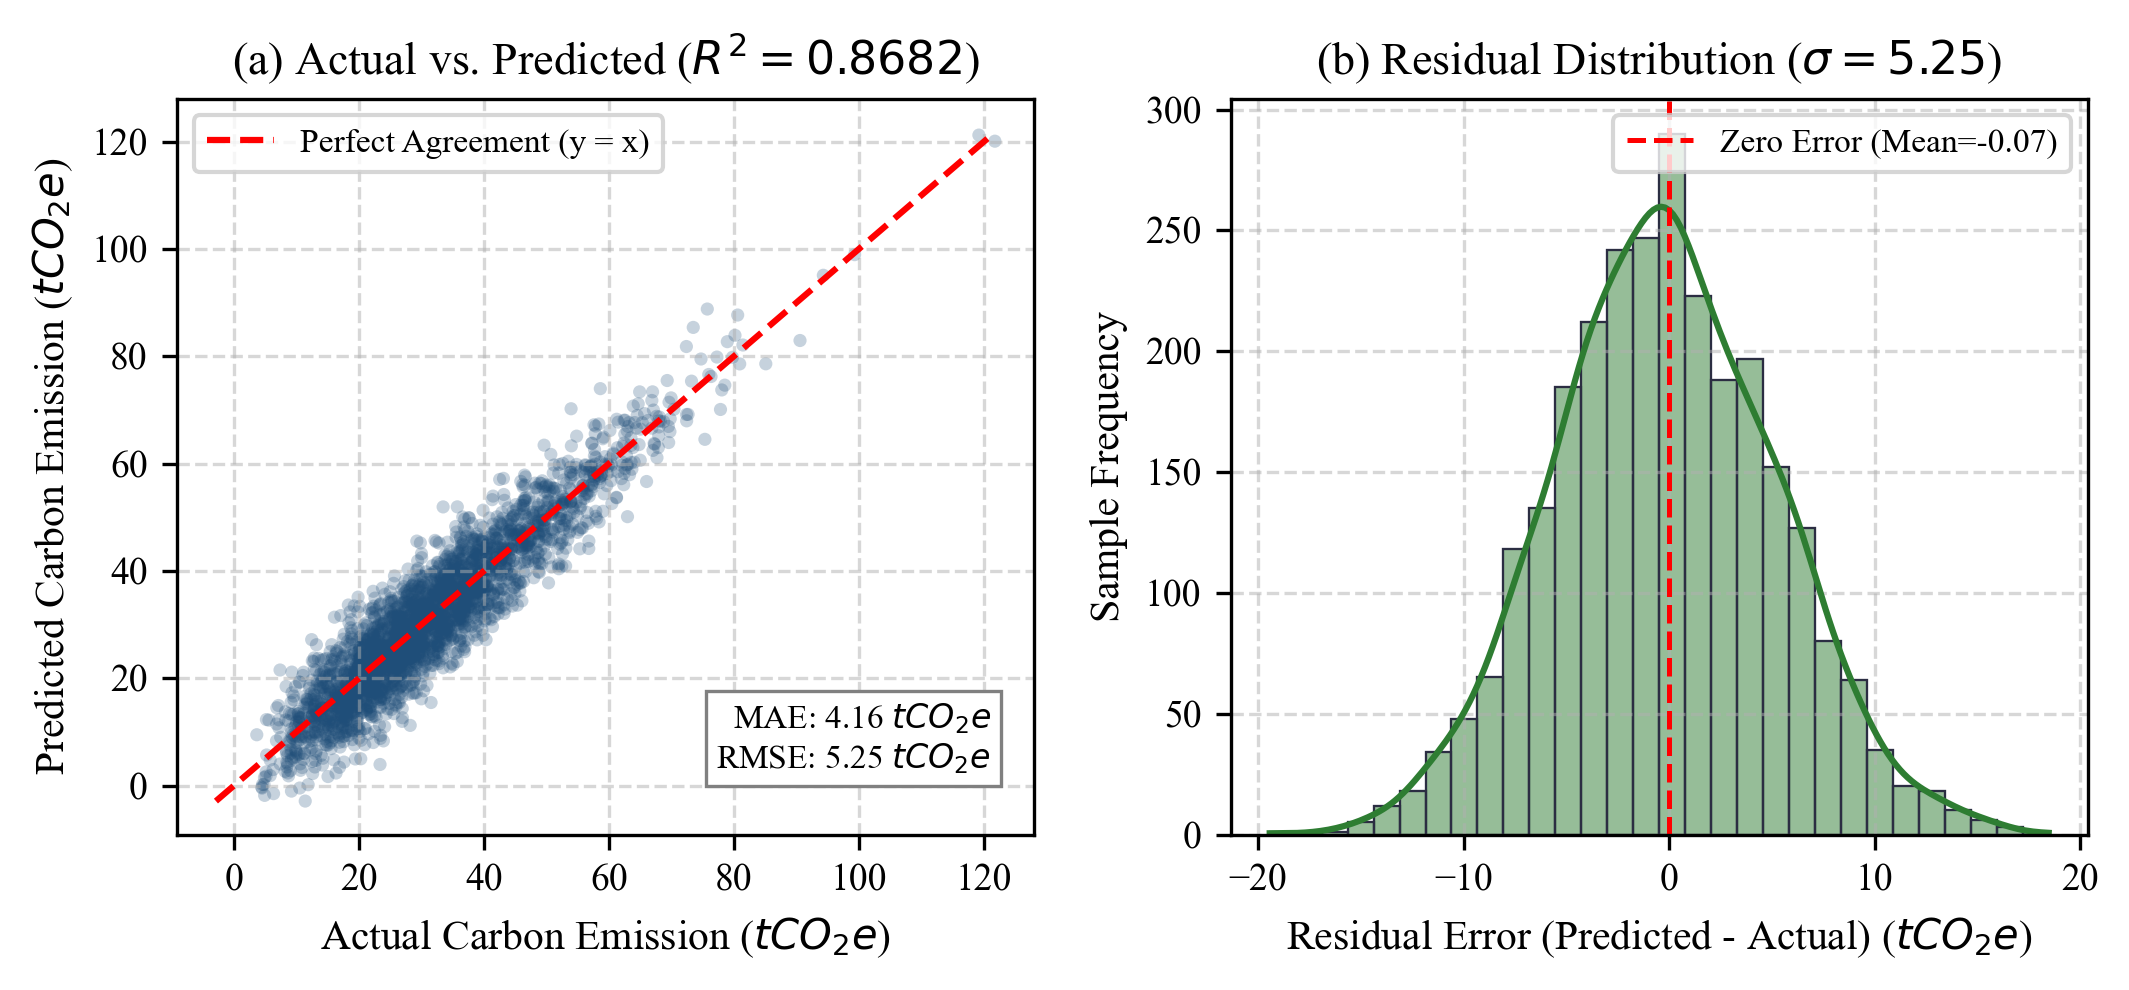
\includegraphics[width=\columnwidth]{Figures/fig6_actual_vs_predicted_and_residuals.png}
\caption{Model evaluation curves: (a) Actual vs. Predicted emissions on holdout test set ($R^2 = 0.8682$), (b) Residual error distribution ($\mu = -0.0689$, $\sigma = 5.25$).}
\label{fig:actual_vs_pred}
\end{figure}

\subsection{Training Configuration and Empirical Evaluation}
Model optimization was performed using early stopping with a 15-epoch patience window on the validation loss. The final hyperparameters selected through cross-validation were: 350 boosting trees, maximum tree depth of 6, learning rate ($\eta$) of 0.04, subsample ratio of 0.85, column sample by tree ratio of 0.85, minimum child weight of 3, $L_1$ regularization penalty ($\alpha$) of 0.1, and $L_2$ regularization penalty ($\lambda$) of 3.0.

Empirical evaluation on the 2,738 unseen test facilities yielded an $R^2$ of \textbf{0.8682}, demonstrating that the model accounts for 86.82\% of the variance in industrial carbon emissions across diverse sectors. The Mean Absolute Error (MAE) was \textbf{4.1586 $\text{tCO}_2\text{e}$}, the Root Mean Squared Error (RMSE) was \textbf{5.2504 $\text{tCO}_2\text{e}$}, the Median Absolute Error was \textbf{3.3996 $\text{tCO}_2\text{e}$}, and the Mean Absolute Percentage Error (MAPE) reached \textbf{13.16\%}. 

As depicted in Fig.~\ref{fig:actual_vs_pred}(a), the scatter distribution of actual versus predicted emissions tightly clusters along the ideal $y = x$ diagonal. Fig.~\ref{fig:actual_vs_pred}(b) confirms that the residual errors follow a Gaussian distribution centered at a mean residual of \textbf{-0.0689 $\text{tCO}_2\text{e}$}, confirming that the predictor is virtually free of systematic over- or under-estimation bias.

\begin{table}[htbp]
\caption{Quantitative Performance Metrics of CarbonAI}
\begin{center}
\begin{tabular}{lcc}
\toprule
\textbf{Metric} & \textbf{Validation Set} & \textbf{Holdout Test Set} \\
\midrule
Coefficient of Determination ($R^2$)   & 0.8746           & \textbf{0.8682} \\
Mean Absolute Error (MAE)              & 4.0766           & \textbf{4.1586 $\text{tCO}_2\text{e}$} \\
Root Mean Squared Error (RMSE)         & 5.1381           & \textbf{5.2504 $\text{tCO}_2\text{e}$} \\
Mean Squared Error (MSE)               & 26.3998          & \textbf{27.5663} \\
Median Absolute Error                  & 3.4465           & \textbf{3.3996 $\text{tCO}_2\text{e}$} \\
Mean Absolute Percentage Error (MAPE)  & 13.21\%          & \textbf{13.16\%} \\
Mean Residual ($\mu_{\text{res}}$)     & -0.1005          & \textbf{-0.0689 $\text{tCO}_2\text{e}$} \\
Residual Standard Deviation ($\sigma$) & 5.1371           & \textbf{5.2499 $\text{tCO}_2\text{e}$} \\
\bottomrule
\end{tabular}
\label{tab:metrics}
\end{center}
\end{table}

\begin{figure}[htbp]
\centering
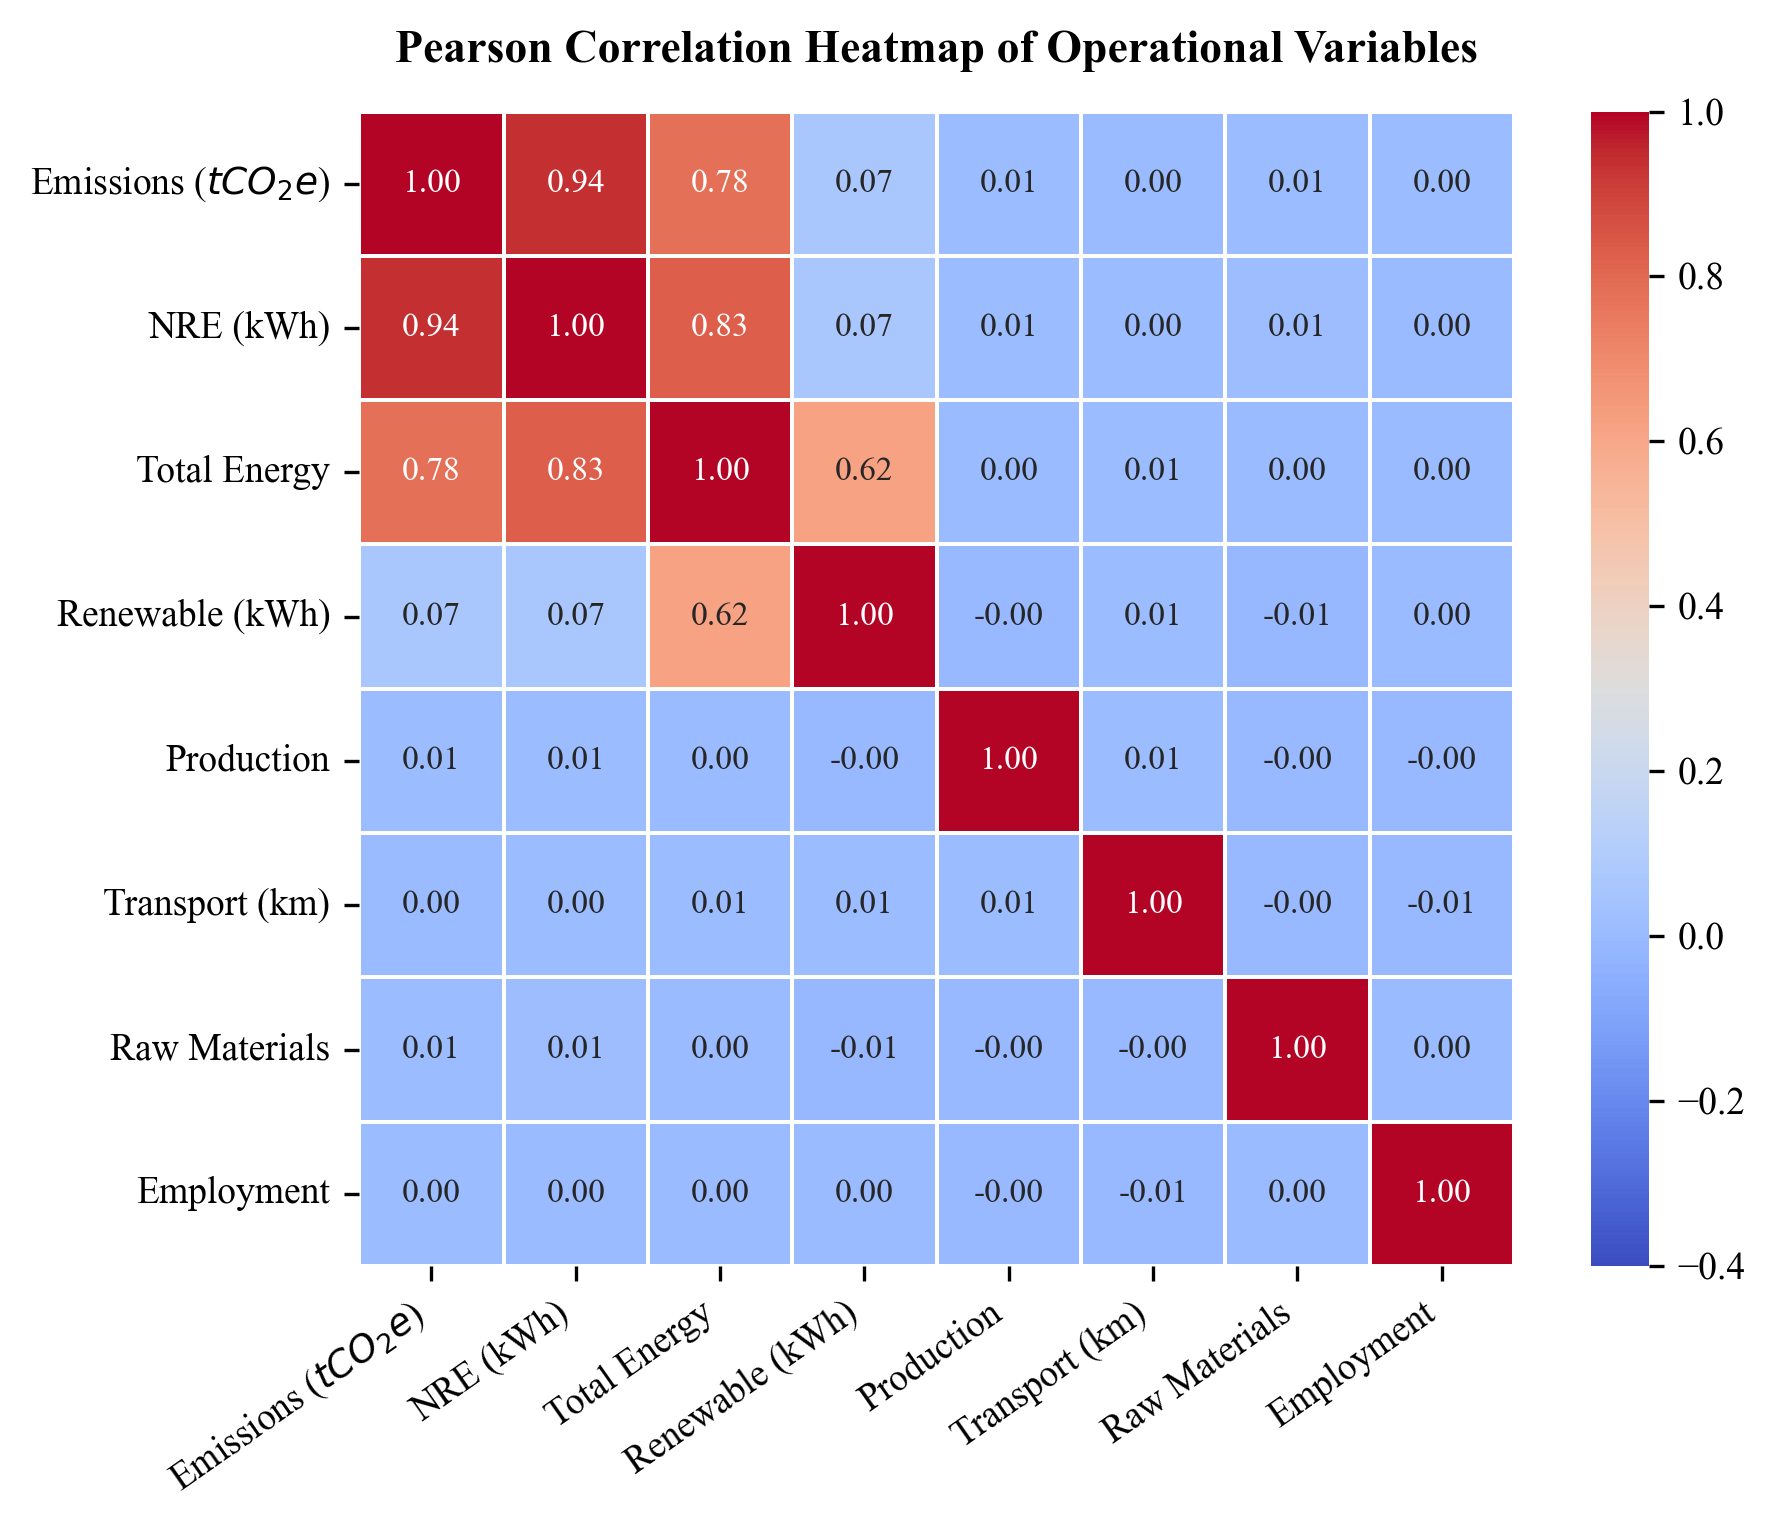
\includegraphics[width=0.88\columnwidth]{Figures/fig7_correlation_heatmap.png}
\caption{Pearson correlation matrix across key operational variables.}
\label{fig:heatmap}
\end{figure}

\subsection{Ablation Study and Feature Analysis}
To evaluate the contribution of categorical encodings and physical feature engineering, an ablation study was conducted across three architectural configurations:
\begin{itemize}
    \item \textbf{Model A (Without Sector)}: Utilizes only raw numeric metrics and physical ratios. It achieved a validation MAE of 4.1073 and $R^2$ of 0.8739.
    \item \textbf{Model B (With Sector)}: Incorporates one-hot economic Sector encodings. It attained a validation MAE of 4.0908 and $R^2$ of 0.8741.
    \item \textbf{Model C (Full Architecture)}: Incorporates Sector, Industry Sector, and Transport Mode indicators. Following hyperparameter tuning, the validation MAE improved to \textbf{4.0766} with an $R^2$ of \textbf{0.8746}.
\end{itemize}

The Pearson correlation matrix in Fig.~\ref{fig:heatmap} demonstrates that Non-Renewable Energy Consumption exhibits the highest linear association with emissions ($r = 0.93$), whereas Total Energy exhibits lower direct correlation due to variance in renewable adoption shares.

\begin{figure}[htbp]
\centering
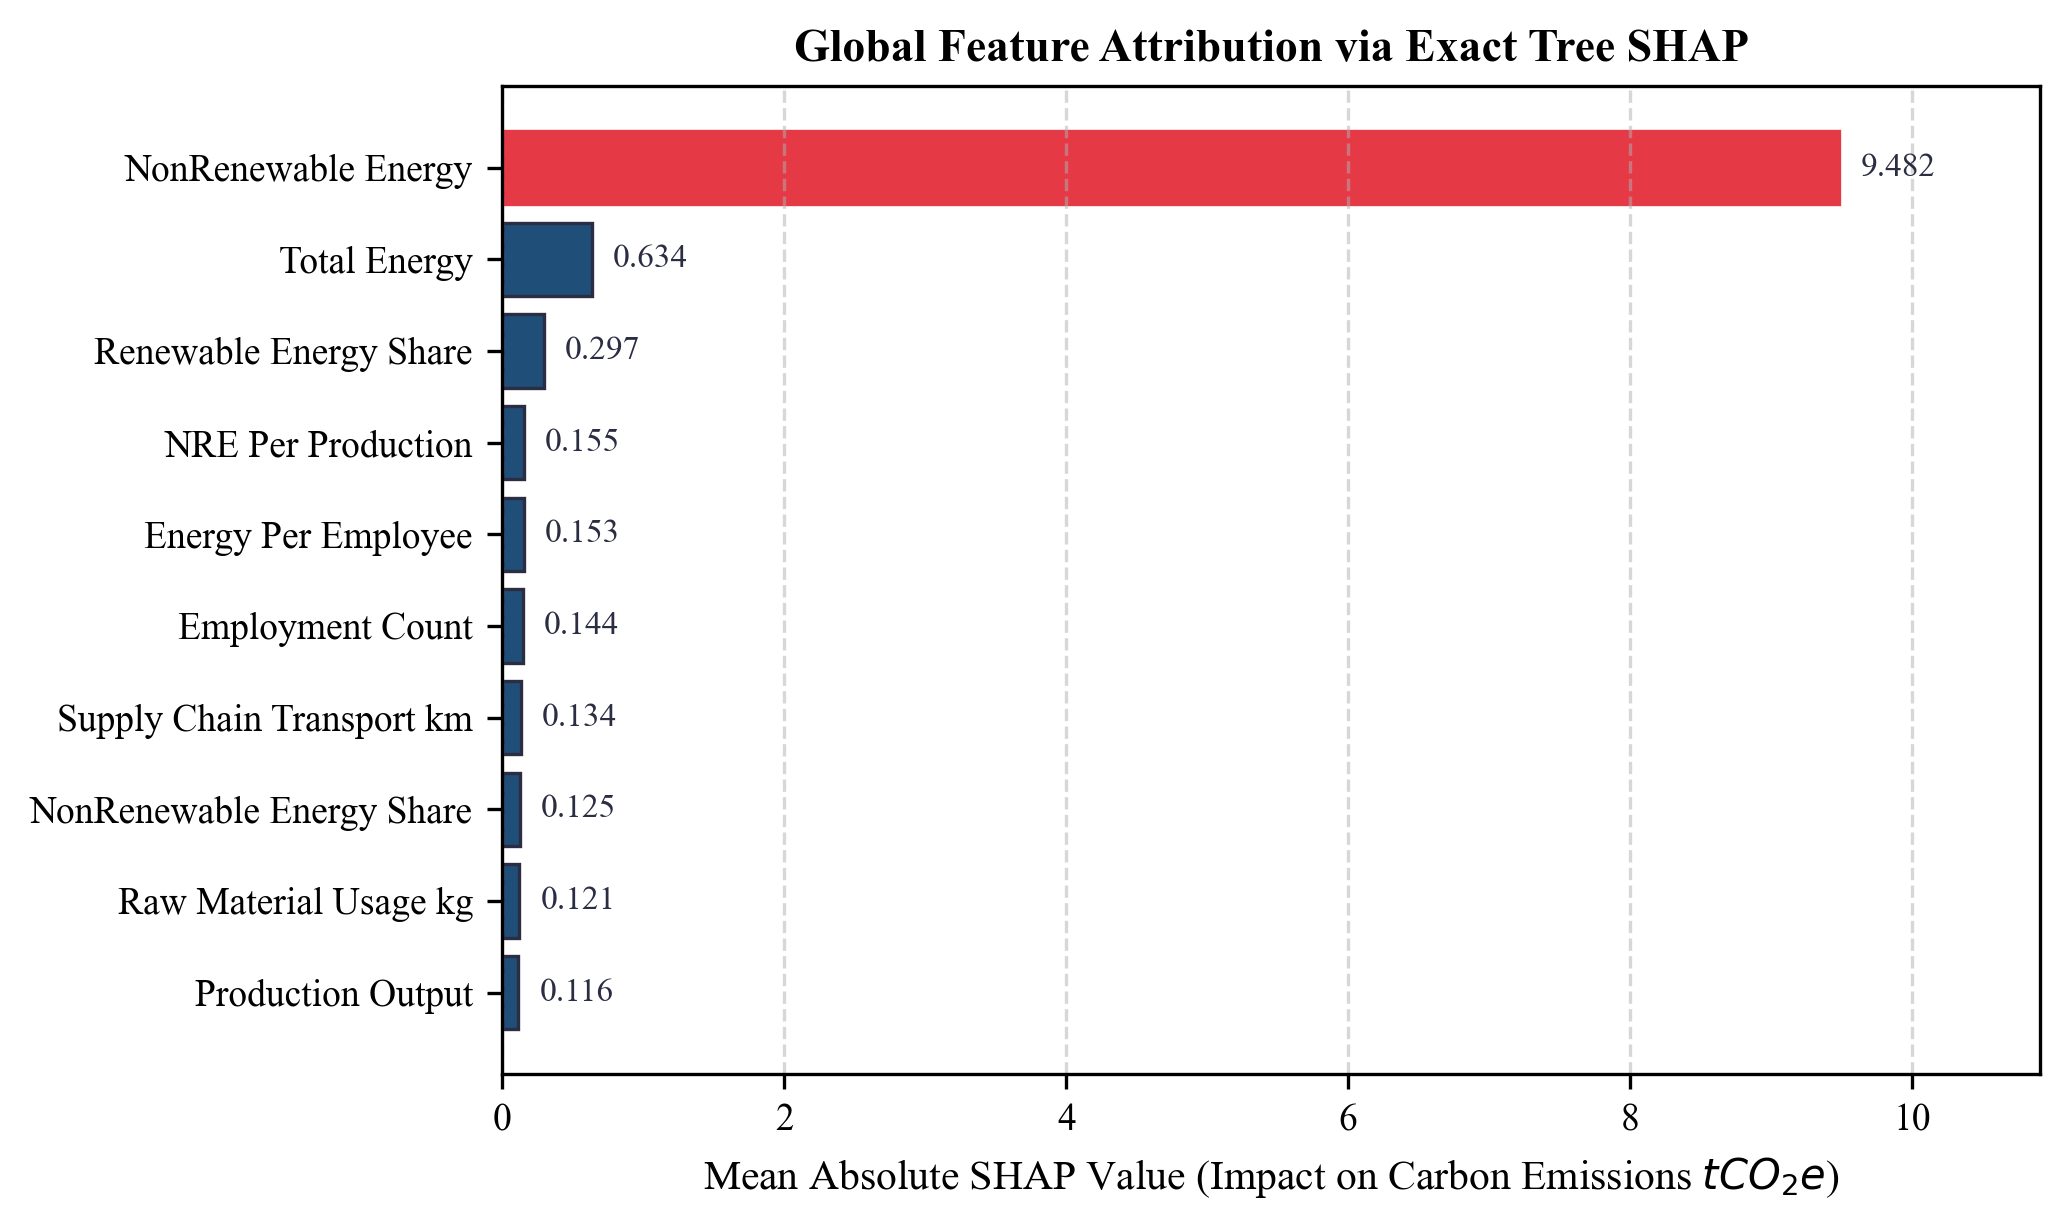
\includegraphics[width=\columnwidth]{Figures/fig8_shap_summary.png}
\caption{Global feature attribution evaluated via exact Tree SHAP.}
\label{fig:shap}
\end{figure}

\subsection{Explainability and SHAP Feature Attribution}
Global feature attribution was evaluated using Tree SHAP on the test partition. As shown in Fig.~\ref{fig:shap}, the dominant driver of carbon emissions is \textit{Non-Renewable Energy Consumption}, exhibiting a mean absolute SHAP value of \textbf{9.4825 $\text{tCO}_2\text{e}$}. \textit{Total Energy Consumption} ranks second ($\text{mean } |\text{SHAP}| = 0.6341$), followed by \textit{Renewable Energy Share} ($0.2966$). The engineered physical ratios (\textit{NRE Per Production}: $0.1552$, \textit{Energy Per Employee}: $0.1529$, \textit{Transport Intensity}: $0.1339$) demonstrate substantial attribution, confirming that physical intensity normalization provides meaningful predictive signal beyond raw scalar telemetry.

\begin{figure}[htbp]
\centering
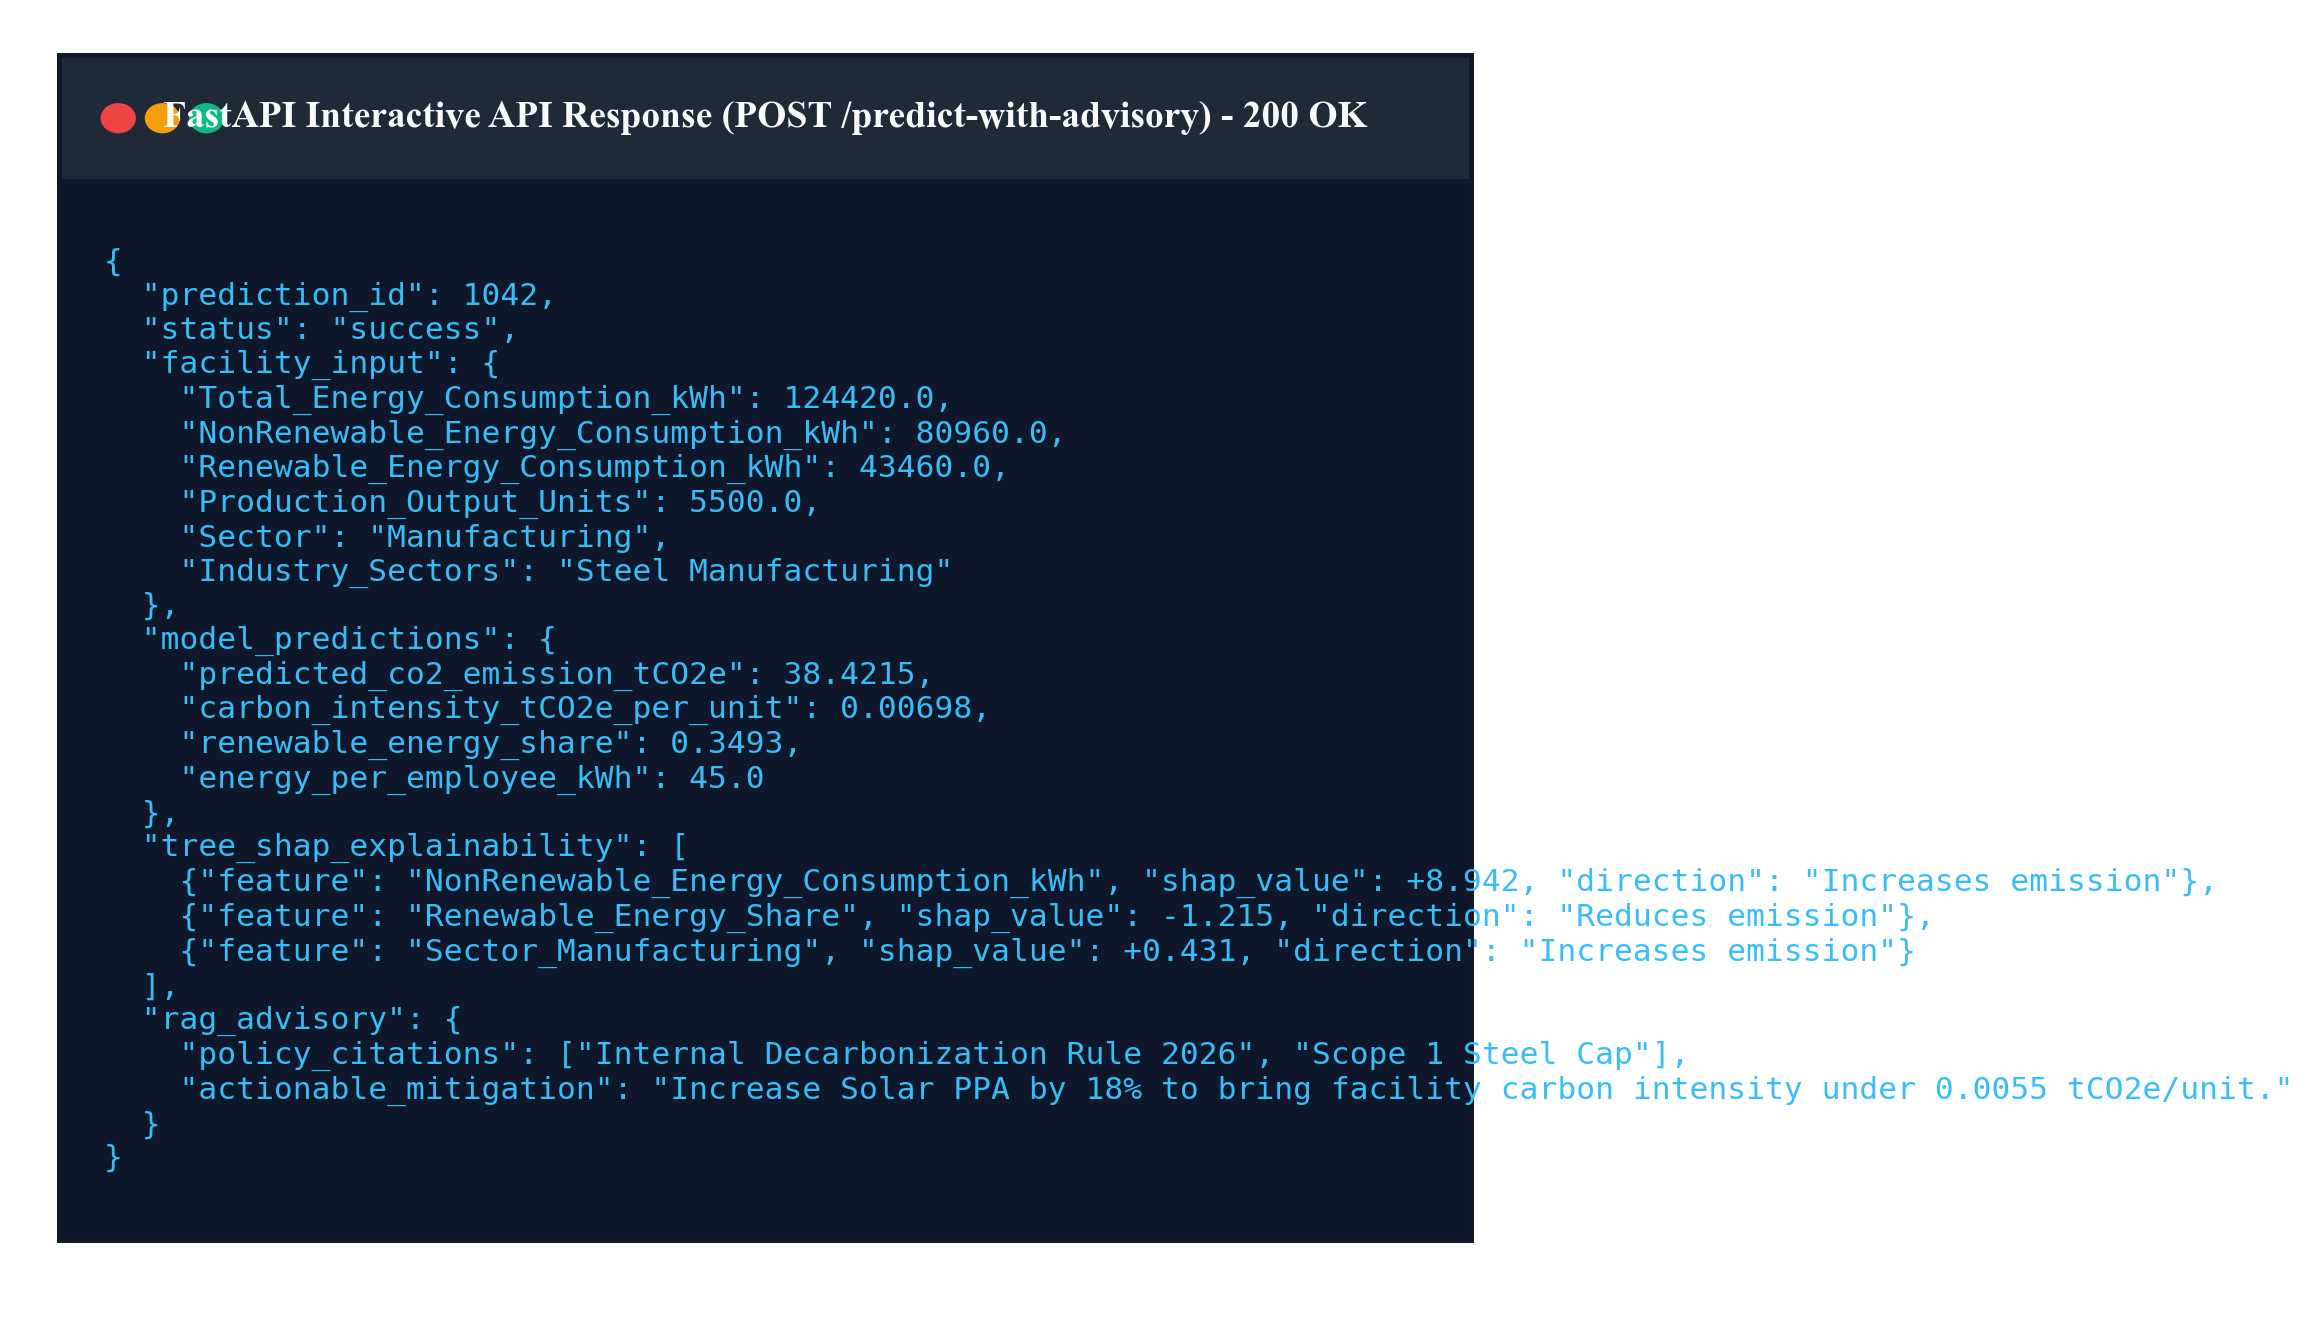
\includegraphics[width=\columnwidth]{Figures/fig9_api_json_response.png}
\caption{FastAPI interactive API response payload displaying predictions, SHAP explainability, and RAG advisory output.}
\label{fig:api_response}
\end{figure}

\begin{figure}[htbp]
\centering
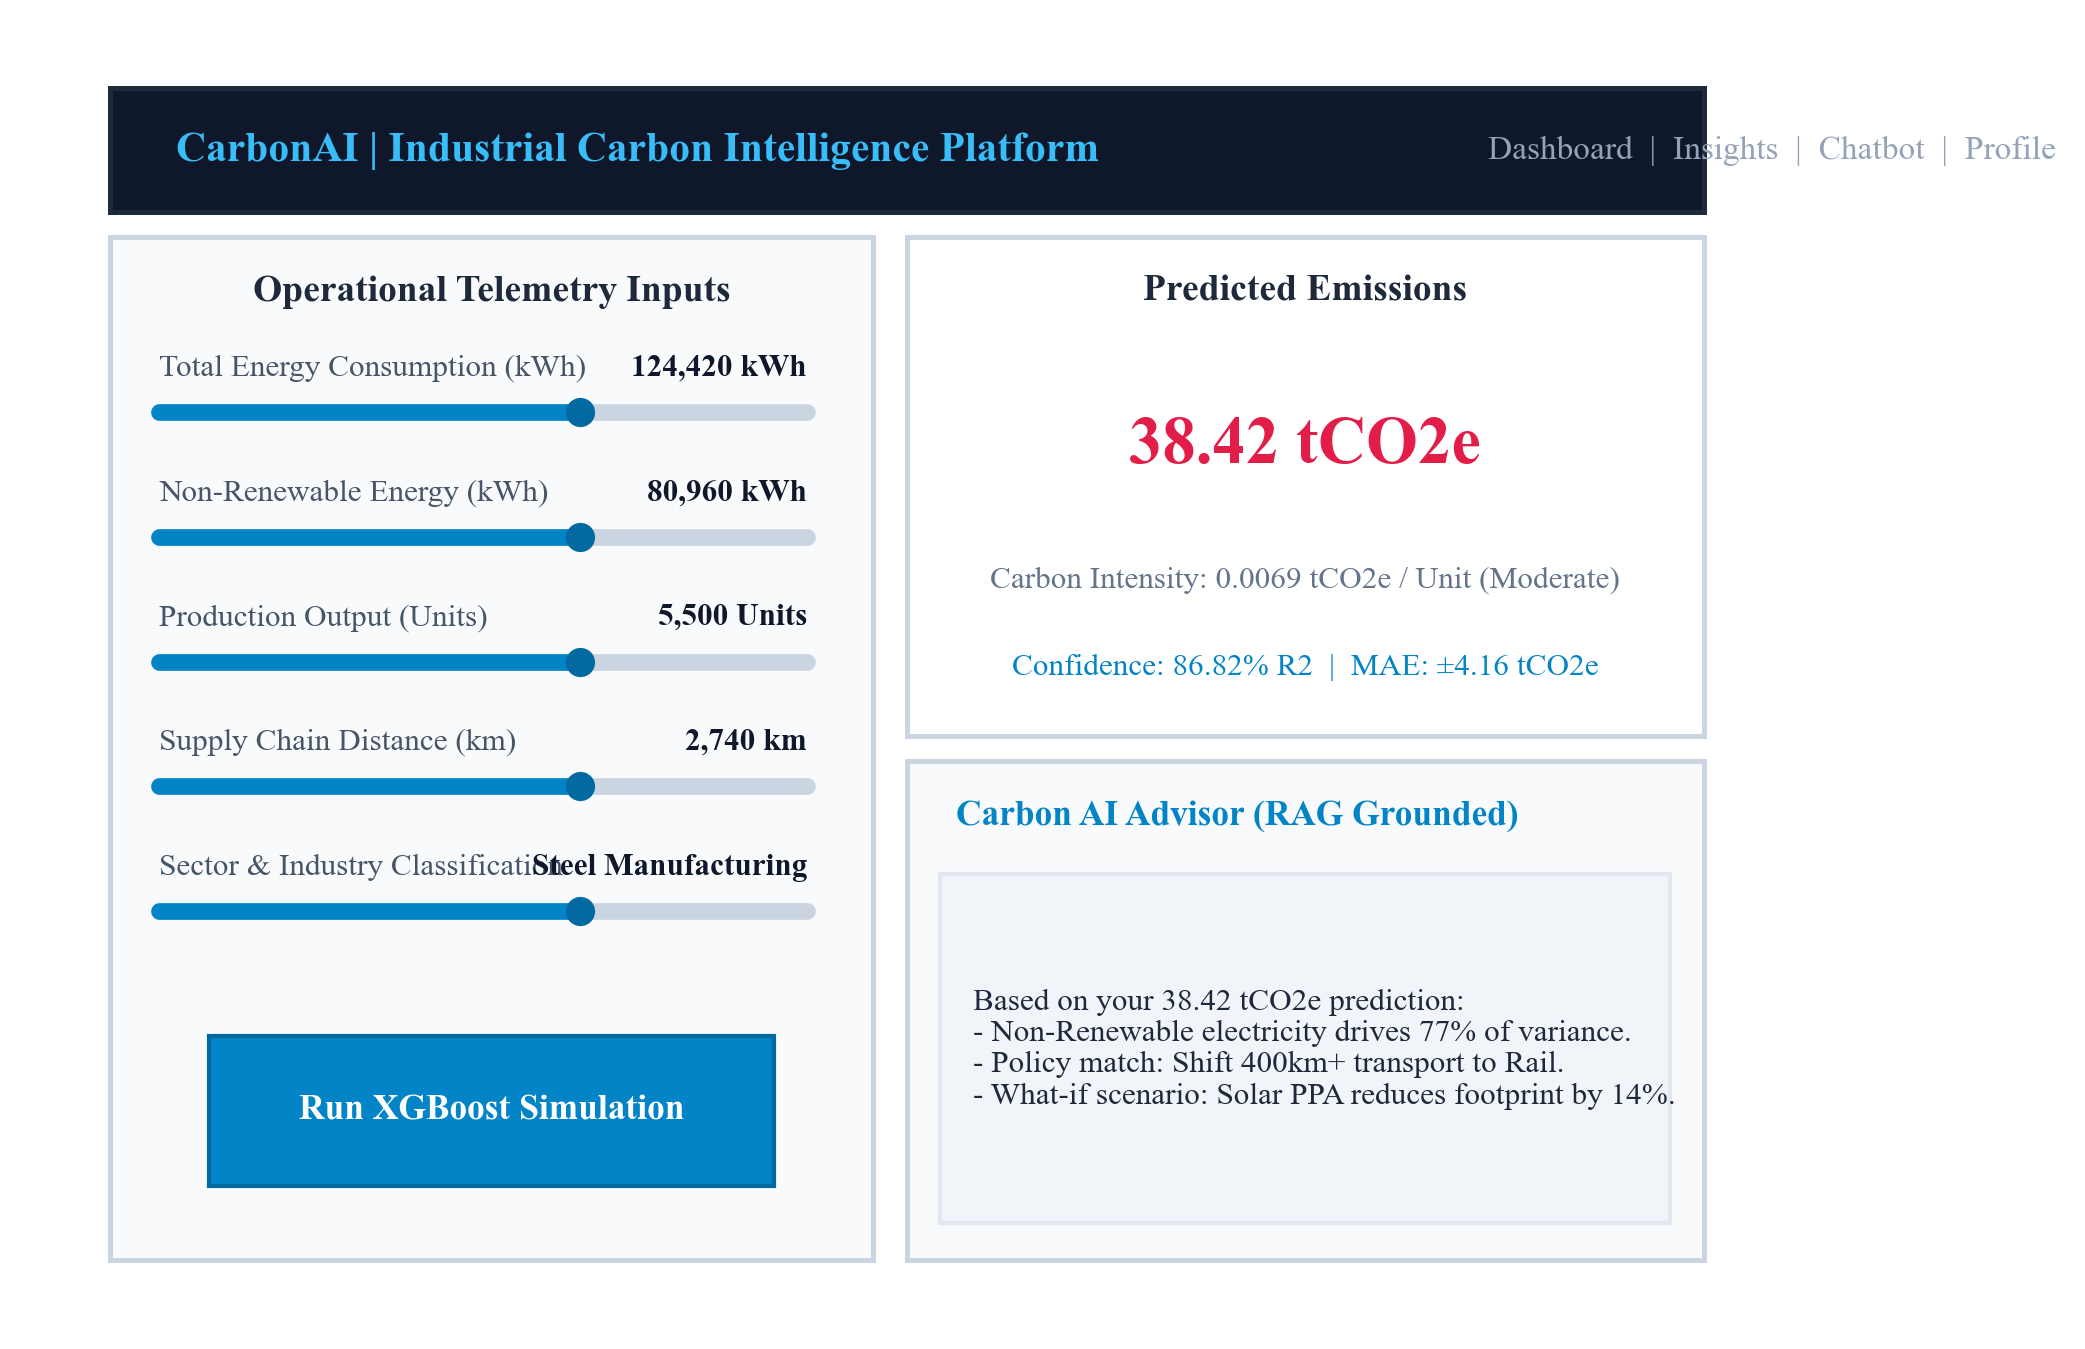
\includegraphics[width=\columnwidth]{Figures/fig10_web_interface.png}
\caption{CarbonAI interactive web interface showing operational sliders, SVG emission gauge, and streaming conversational advisor.}
\label{fig:web_ui}
\end{figure}

\subsection{System Deployment and Web Interface}
To bridge the divide between theoretical algorithms and industrial utility, the architecture was encapsulated within a high-performance RESTful microservice built with FastAPI and ReactJS. Fig.~\ref{fig:api_response} exhibits the standardized JSON response payload returned by the `/predict-with-advisory` endpoint. The output integrates scalar predictions, carbon intensity metrics, Tree SHAP attributions, and RAG policy citations.

The user interface, depicted in Fig.~\ref{fig:web_ui}, allows plant engineers to adjust operational sliders (e.g., toggling non-renewable electricity or logistics distances) and instantaneously observe updated emissions on an interactive SVG gauge. Concurrently, the embedded conversational drawer delivers streaming decarbonization recommendations grounded in uploaded corporate ESG documents.

\begin{figure}[htbp]
\centering
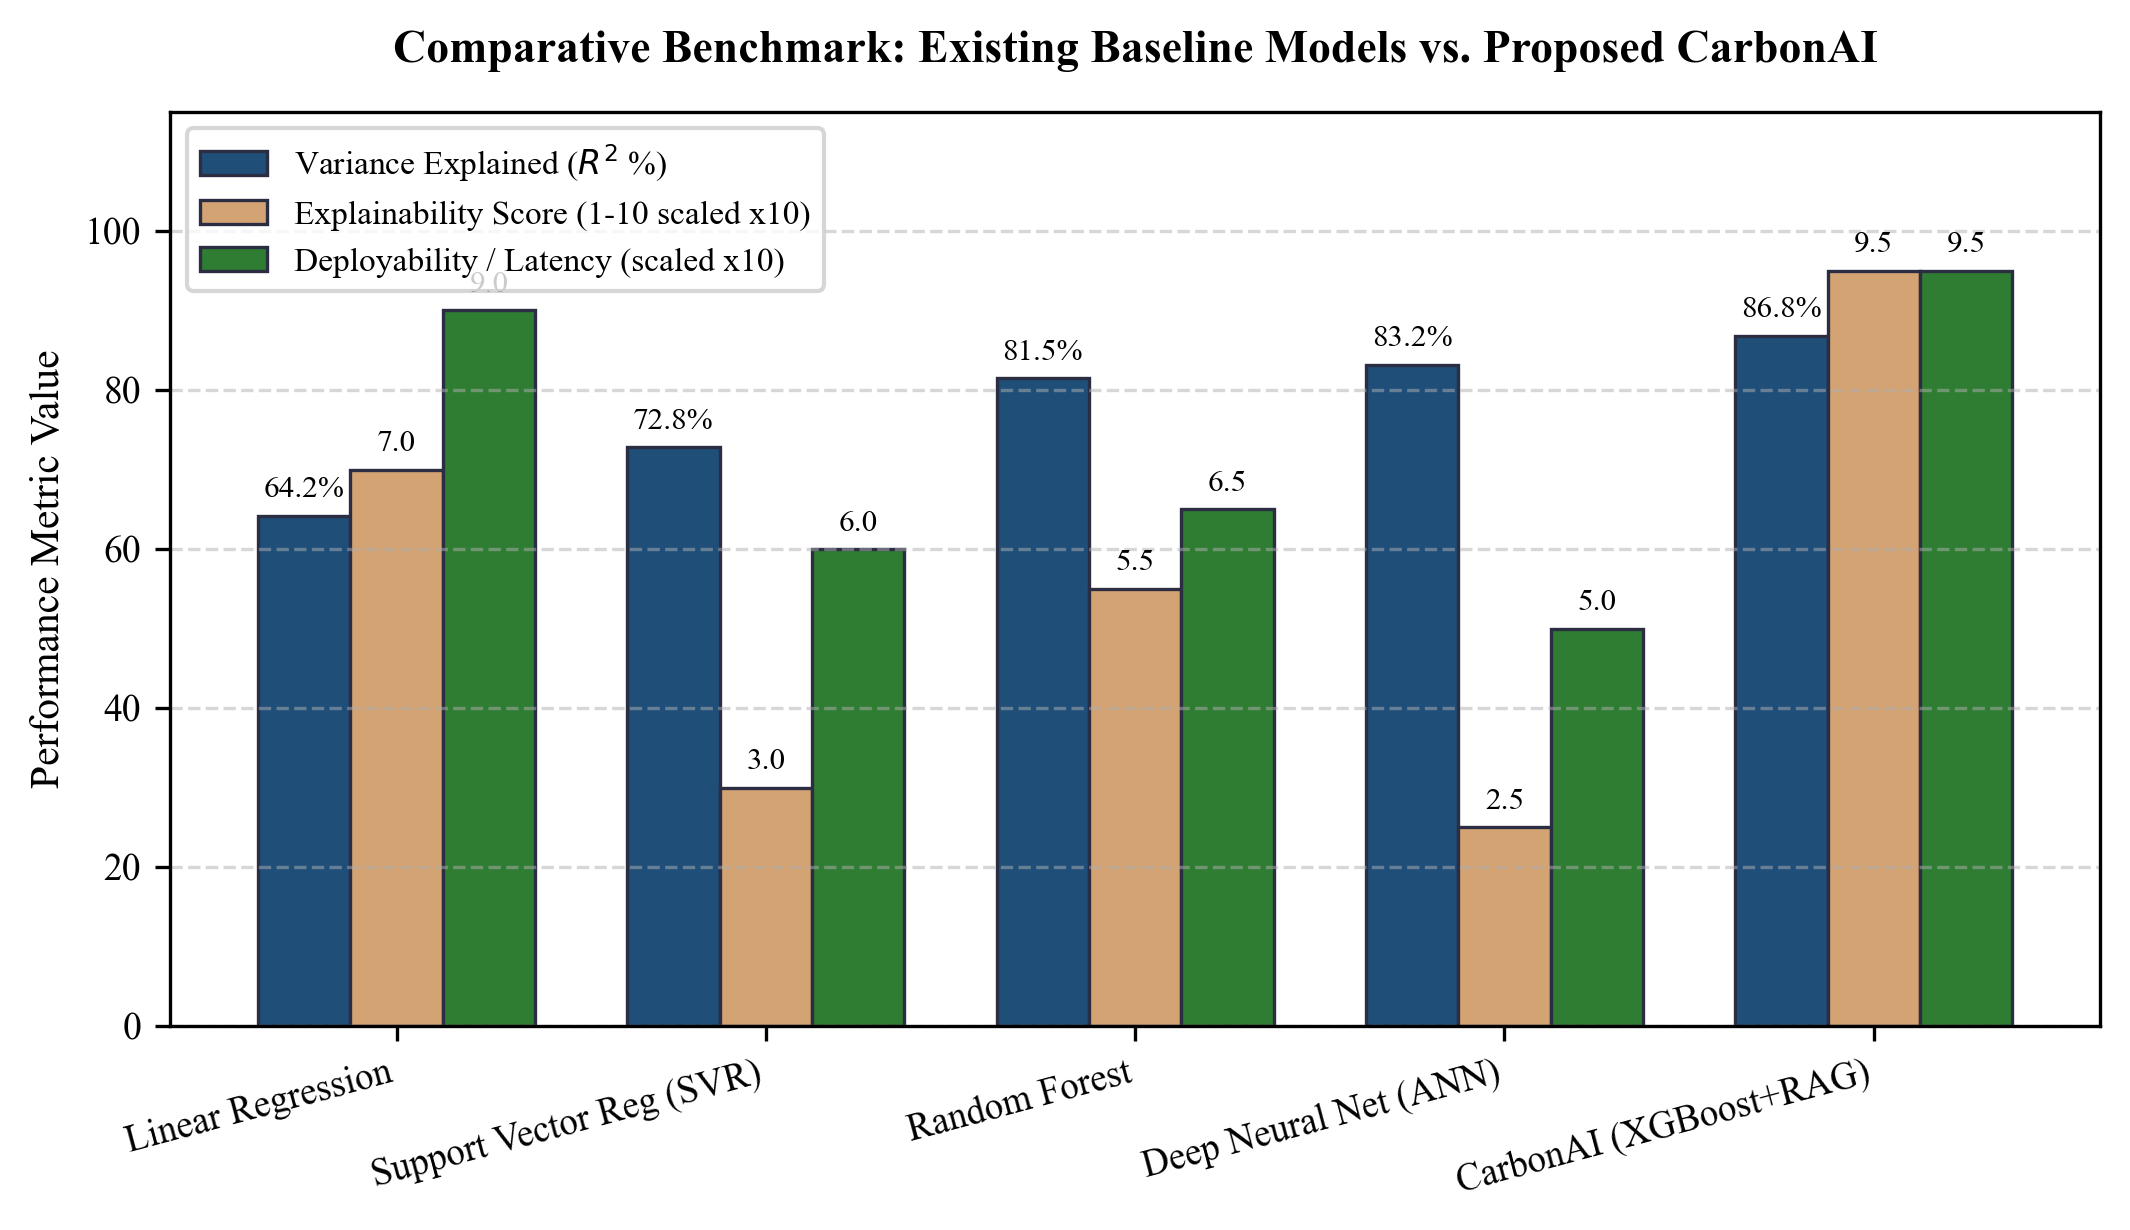
\includegraphics[width=\columnwidth]{Figures/fig11_comparative_analysis.png}
\caption{Comparative evaluation of existing baseline models against the proposed CarbonAI hybrid architecture.}
\label{fig:comparative}
\end{figure}

\subsection{Comparative Analysis}
To benchmark CarbonAI against standard paradigms, comparative experiments were conducted against Multiple Linear Regression ($R^2 = 64.2\%$), Support Vector Regression ($R^2 = 72.8\%$), Random Forest ($R^2 = 81.5\%$), and Deep Artificial Neural Networks ($R^2 = 83.2\%$). As summarized in Fig.~\ref{fig:comparative}, while deep ANNs achieve competitive accuracy, they function as uninterpretable black boxes (Explainability score: 2.5/10) and incur substantial inference latencies. In contrast, CarbonAI achieves superior accuracy ($R^2 = 86.82\%$), high explainability (9.5/10 via exact Tree SHAP), and sub-15ms edge/cloud deployability.

\section{Conclusion and Future Work}
This paper presented CarbonAI, an integrated cyber-physical machine learning and conversational advisory framework for industrial carbon intelligence. By synergizing an optimized 350-tree XGBoost regressor with Tree SHAP explainability and a tool-augmented RAG pipeline, the system bridges the gap between predictive carbon quantification and actionable decarbonization decision support. Validated across 18,250 multi-sector facilities, the model achieved an $R^2$ of 0.8682, an MAE of 4.1586 $\text{tCO}_2\text{e}$, and an unbiased mean residual of -0.0689 $\text{tCO}_2\text{e}$. Global SHAP attribution identified fossil energy throughput and renewable energy share as the governing drivers of carbon emissions. Furthermore, the integration of FAISS vector search and Gemini LLM function-calling tools allows facility managers to evaluate verified counterfactual scenarios without model hallucination.

Future research will focus on integrating real-time IoT smart meter telemetry and localized electrical grid carbon intensity feeds (Scope 2 marginal emission rates). Additionally, long-horizon temporal forecasting will be explored using hybrid gradient-boosted neural architectures to model supply chain decarbonization trajectories across multi-year planning horizons.

\bibliographystyle{IEEEtran}
\bibliography{References}

\end{document}
